\ifdefined\BuildingFromMainFile
\else
   \documentclass[../main.tex]{subfiles}
   \graphicspath{{figure/}{../figure/}}
   \begin{document}
\fi


\newpage

\setcounter{subsection}{0}
\renewcommand \thesubsection {Note S4.\arabic{subsection}}
\setcounter{figure}{0}
\renewcommand \thefigure {S4.\arabic{figure}}
\setcounter{table}{0}
\renewcommand \thetable {S4.\arabic{table}}

\begin{flushleft}

\begin{figure}[!htb]
    \centering
    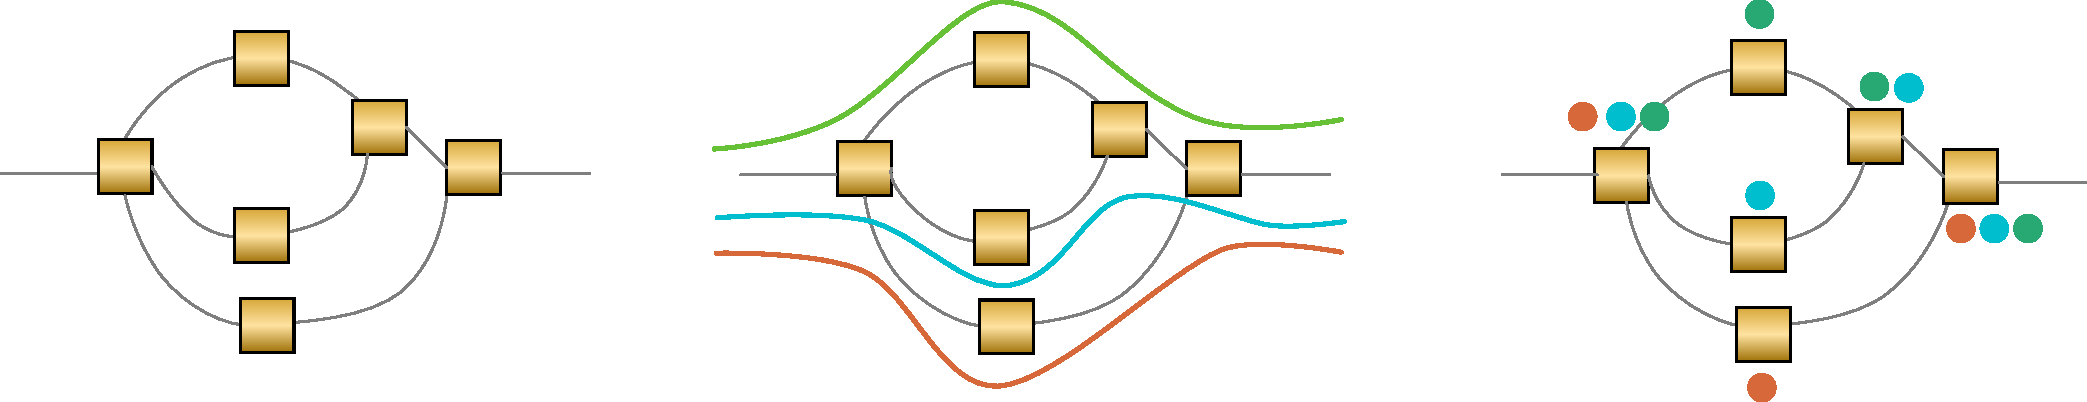
\includegraphics[width=\textwidth]{paper3/supplement/sp41.pdf}
    \caption[Node labelling procedures]{\textbf{Labelling of the nodes in the multi-assembly graph.} \\
    \small{To determine the support for the nodes in the graph, we aligned each individual assembly back to the multi-assembly graph and labeled nodes according to the assembly paths that traversed them with different colors. The left panel represents a schematic graph. Rectangles and lines represent nodes and edges, respectively. The middle panel represents the paths of three assemblies traversing the nodes. The right panel displays how each node that was traversed by an assembly receives a label (colored dots).}}
    \label{sup_fig:s41}
\end{figure}


\newpage

\begin{figure}[!htb]
    \centering
    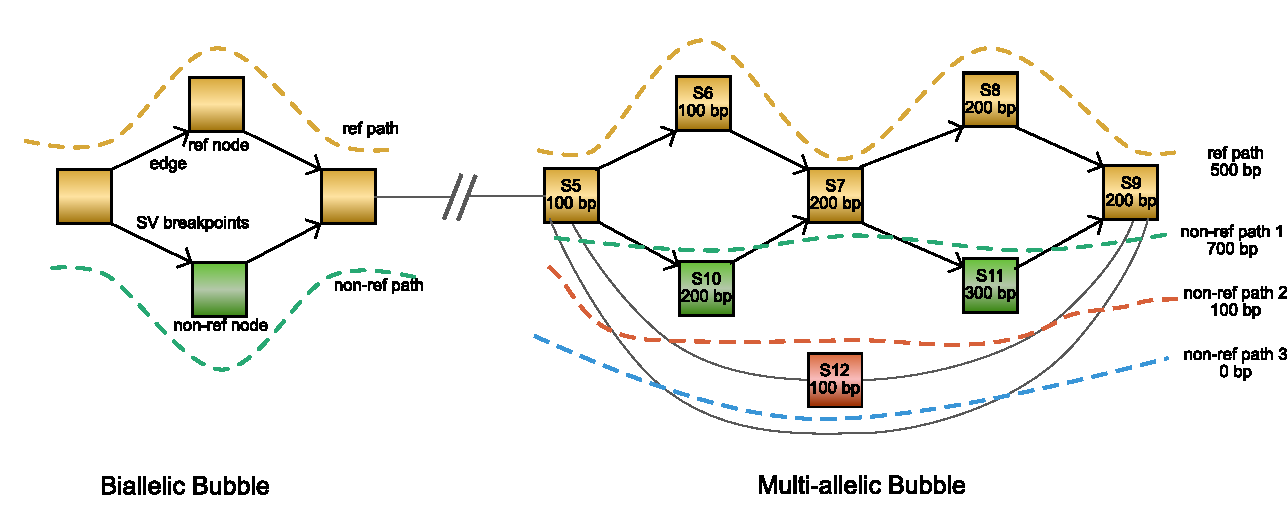
\includegraphics[width=\textwidth]{paper3/supplement/sp42.pdf}
    \caption[SV extraction procedures]{\textbf{Graphs and structural variants terminology used in the paper.} \\
    \small{\emph{(left)} A node contains a sequence of nucleotides (S1-S12). Reference nodes (S1, S2, S4) are derived from the backbone assembly used to construct the graph. Non-reference nodes (S3) contain sequences from additional assemblies that are not present in the backbone. Nodes are connected by directed edges from parent to child where the underlying sequences are contiguous. Edges between reference and non-reference nodes are breakpoints of structural variations. Bubbles are branching regions in the graph which start and end at reference nodes. \emph{(right)} Paths in the bubbles represent different alleles of structural variations, which are biallelic if a bubble contains two paths or multiallelic if it contains more. Nodes within biallelic bubbles represent alleles. Within multi-allelic bubbles, multiple nodes may be part of the same path and thus allele. It is worth noting that not all combinations of nodes within bubbles are real paths found in individual assemblies (e.g., S10-S7-S8). As such, color-consistent nodes within a bubble are stitched together to represent true paths. By comparing reference and non-reference paths, it is possible to determine the type of the structural variations (e.g., non-ref path 1: alternate insertion, path 2: alternate deletion, path 3: complete deletion).}}
    \label{sup_fig:s42}
\end{figure}


\begin{figure}[!htb]
    \centering
    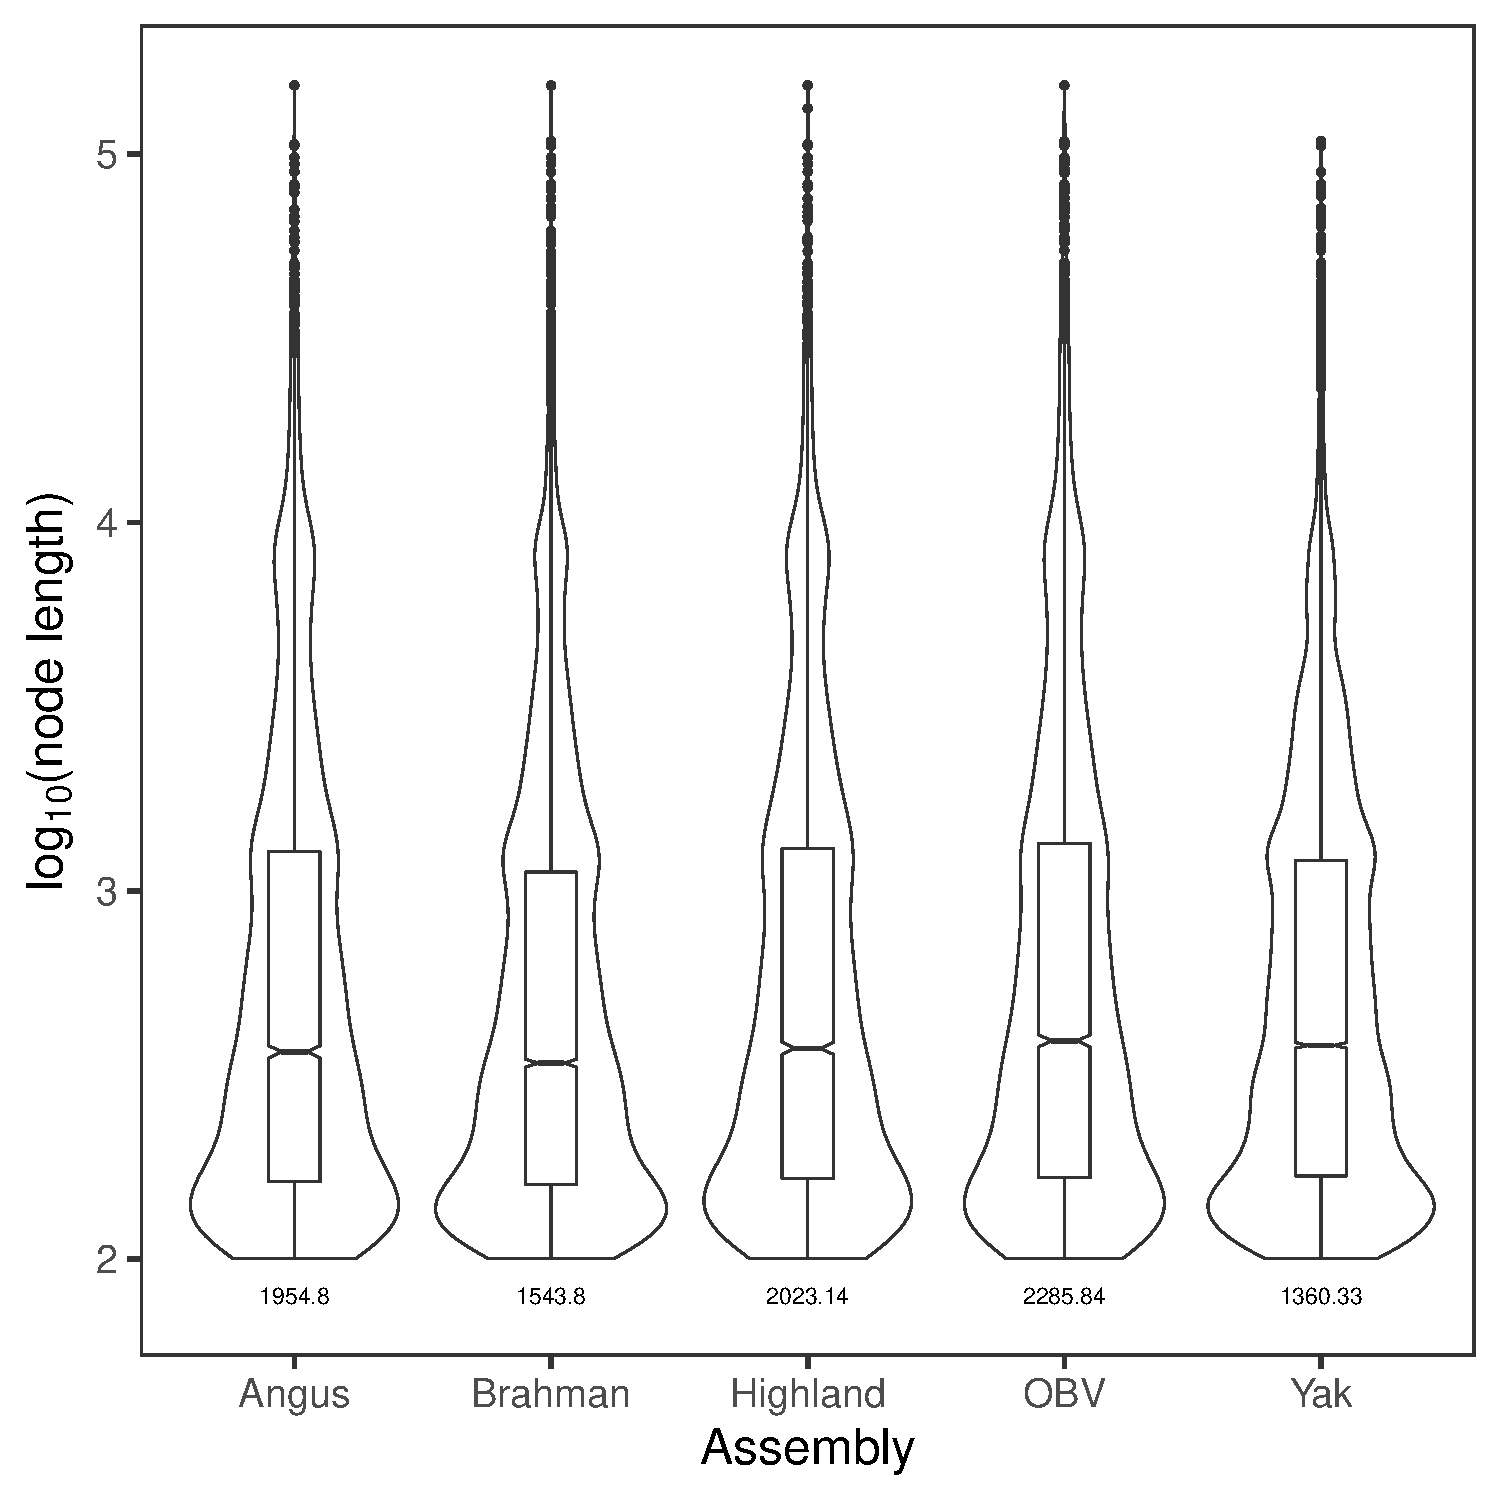
\includegraphics[width=0.7\textwidth]{paper3/supplement/sp43.pdf}
    \caption[Non-reference nodes length]{\textbf{The size of non-reference nodes labelled with each of the five assemblies.} \\
    \small{The Y-axis is log10-scaled. Numbers below each plot refer to the average non-reference node length from each assembly. }}
    \label{sup_fig:s43}
\end{figure}

\newpage

\begin{landscape}
\begin{figure}[!htb]
    \centering
    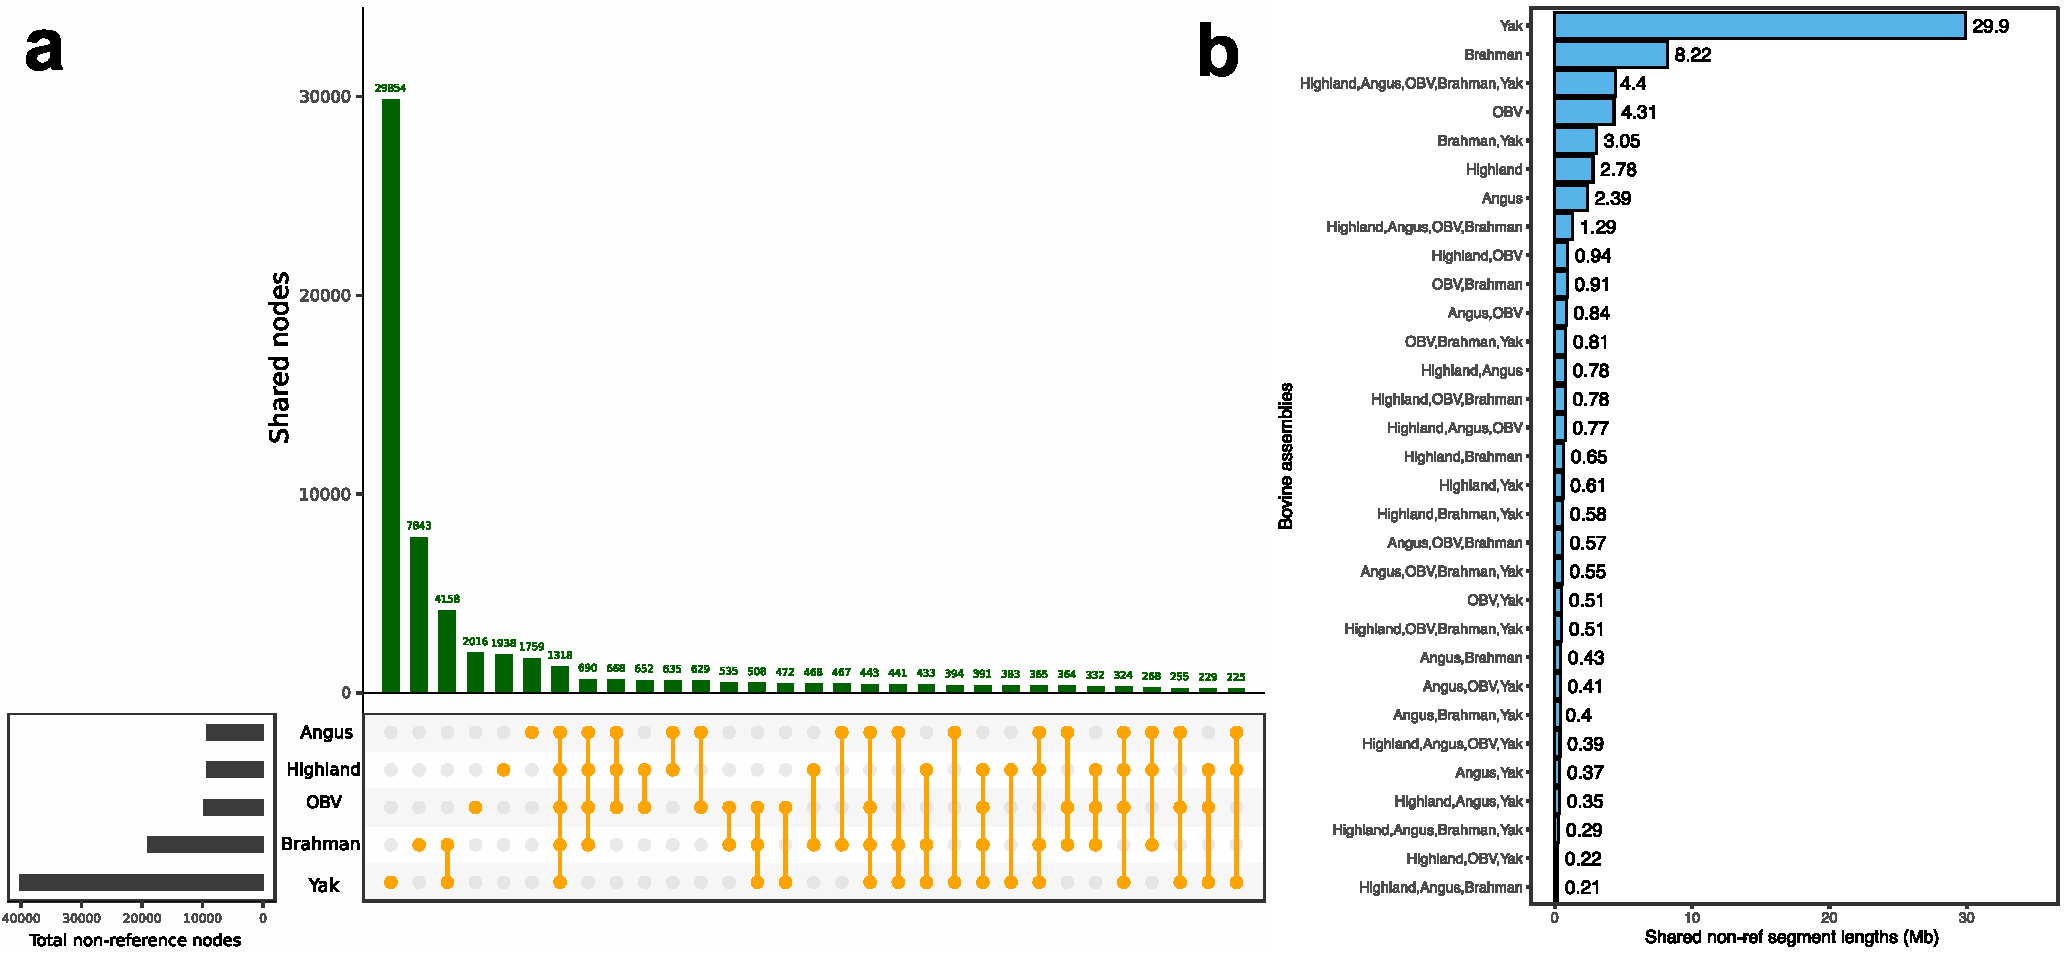
\includegraphics[width=1.5\textwidth]{paper3/supplement/sp44.pdf}
    \caption[Sharing of the non-reference nodes]{\textbf{Non-reference nodes detected across assemblies.} \\
    \small{Intersection of non-reference nodes (a) and cumulative length of non-reference sequences (b) found in five assemblies when compared to ARS-UCD1.2. OBV = Original Braunvieh.}}
    \label{sup_fig:s44}
\end{figure}
\end{landscape}

\newpage


\begin{figure}[!htb]
    \centering
    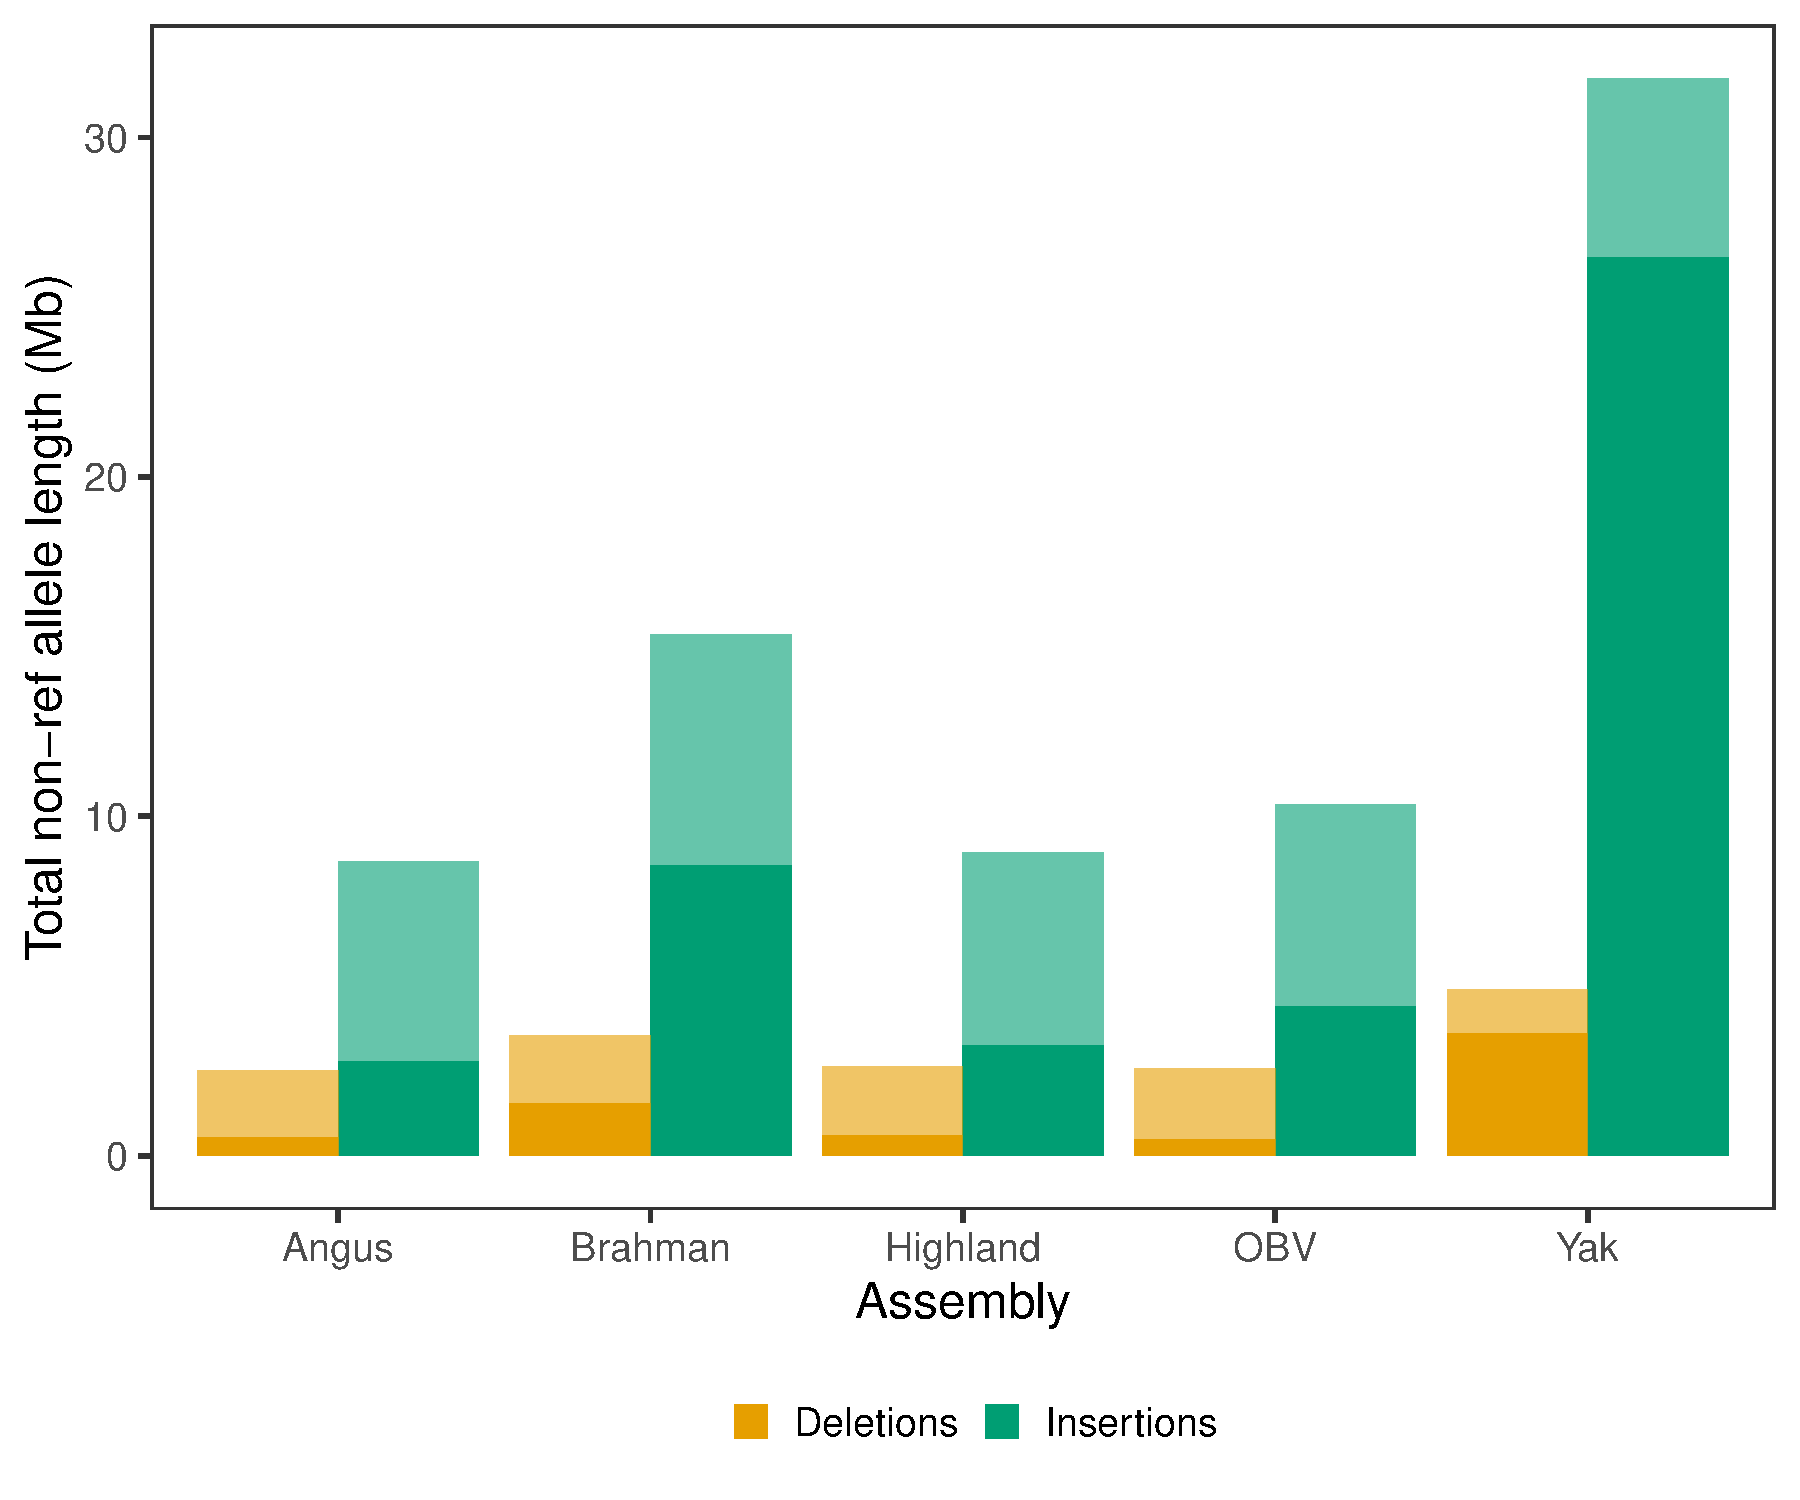
\includegraphics[width=\textwidth]{paper3/supplement/sp45.pdf}
    \caption[Insertions and deletions across breeds]{\textbf{Deletion and insertion polymorphism detected from each assembly in the pangenome graph.} \\
    \small{Transparent and solid bars indicate the total and private length of non-reference alleles respectively. OBV – Original Braunvieh.}}
    \label{sup_fig:s45}
\end{figure}

\newpage

\begin{figure}[!htb]
    \centering
    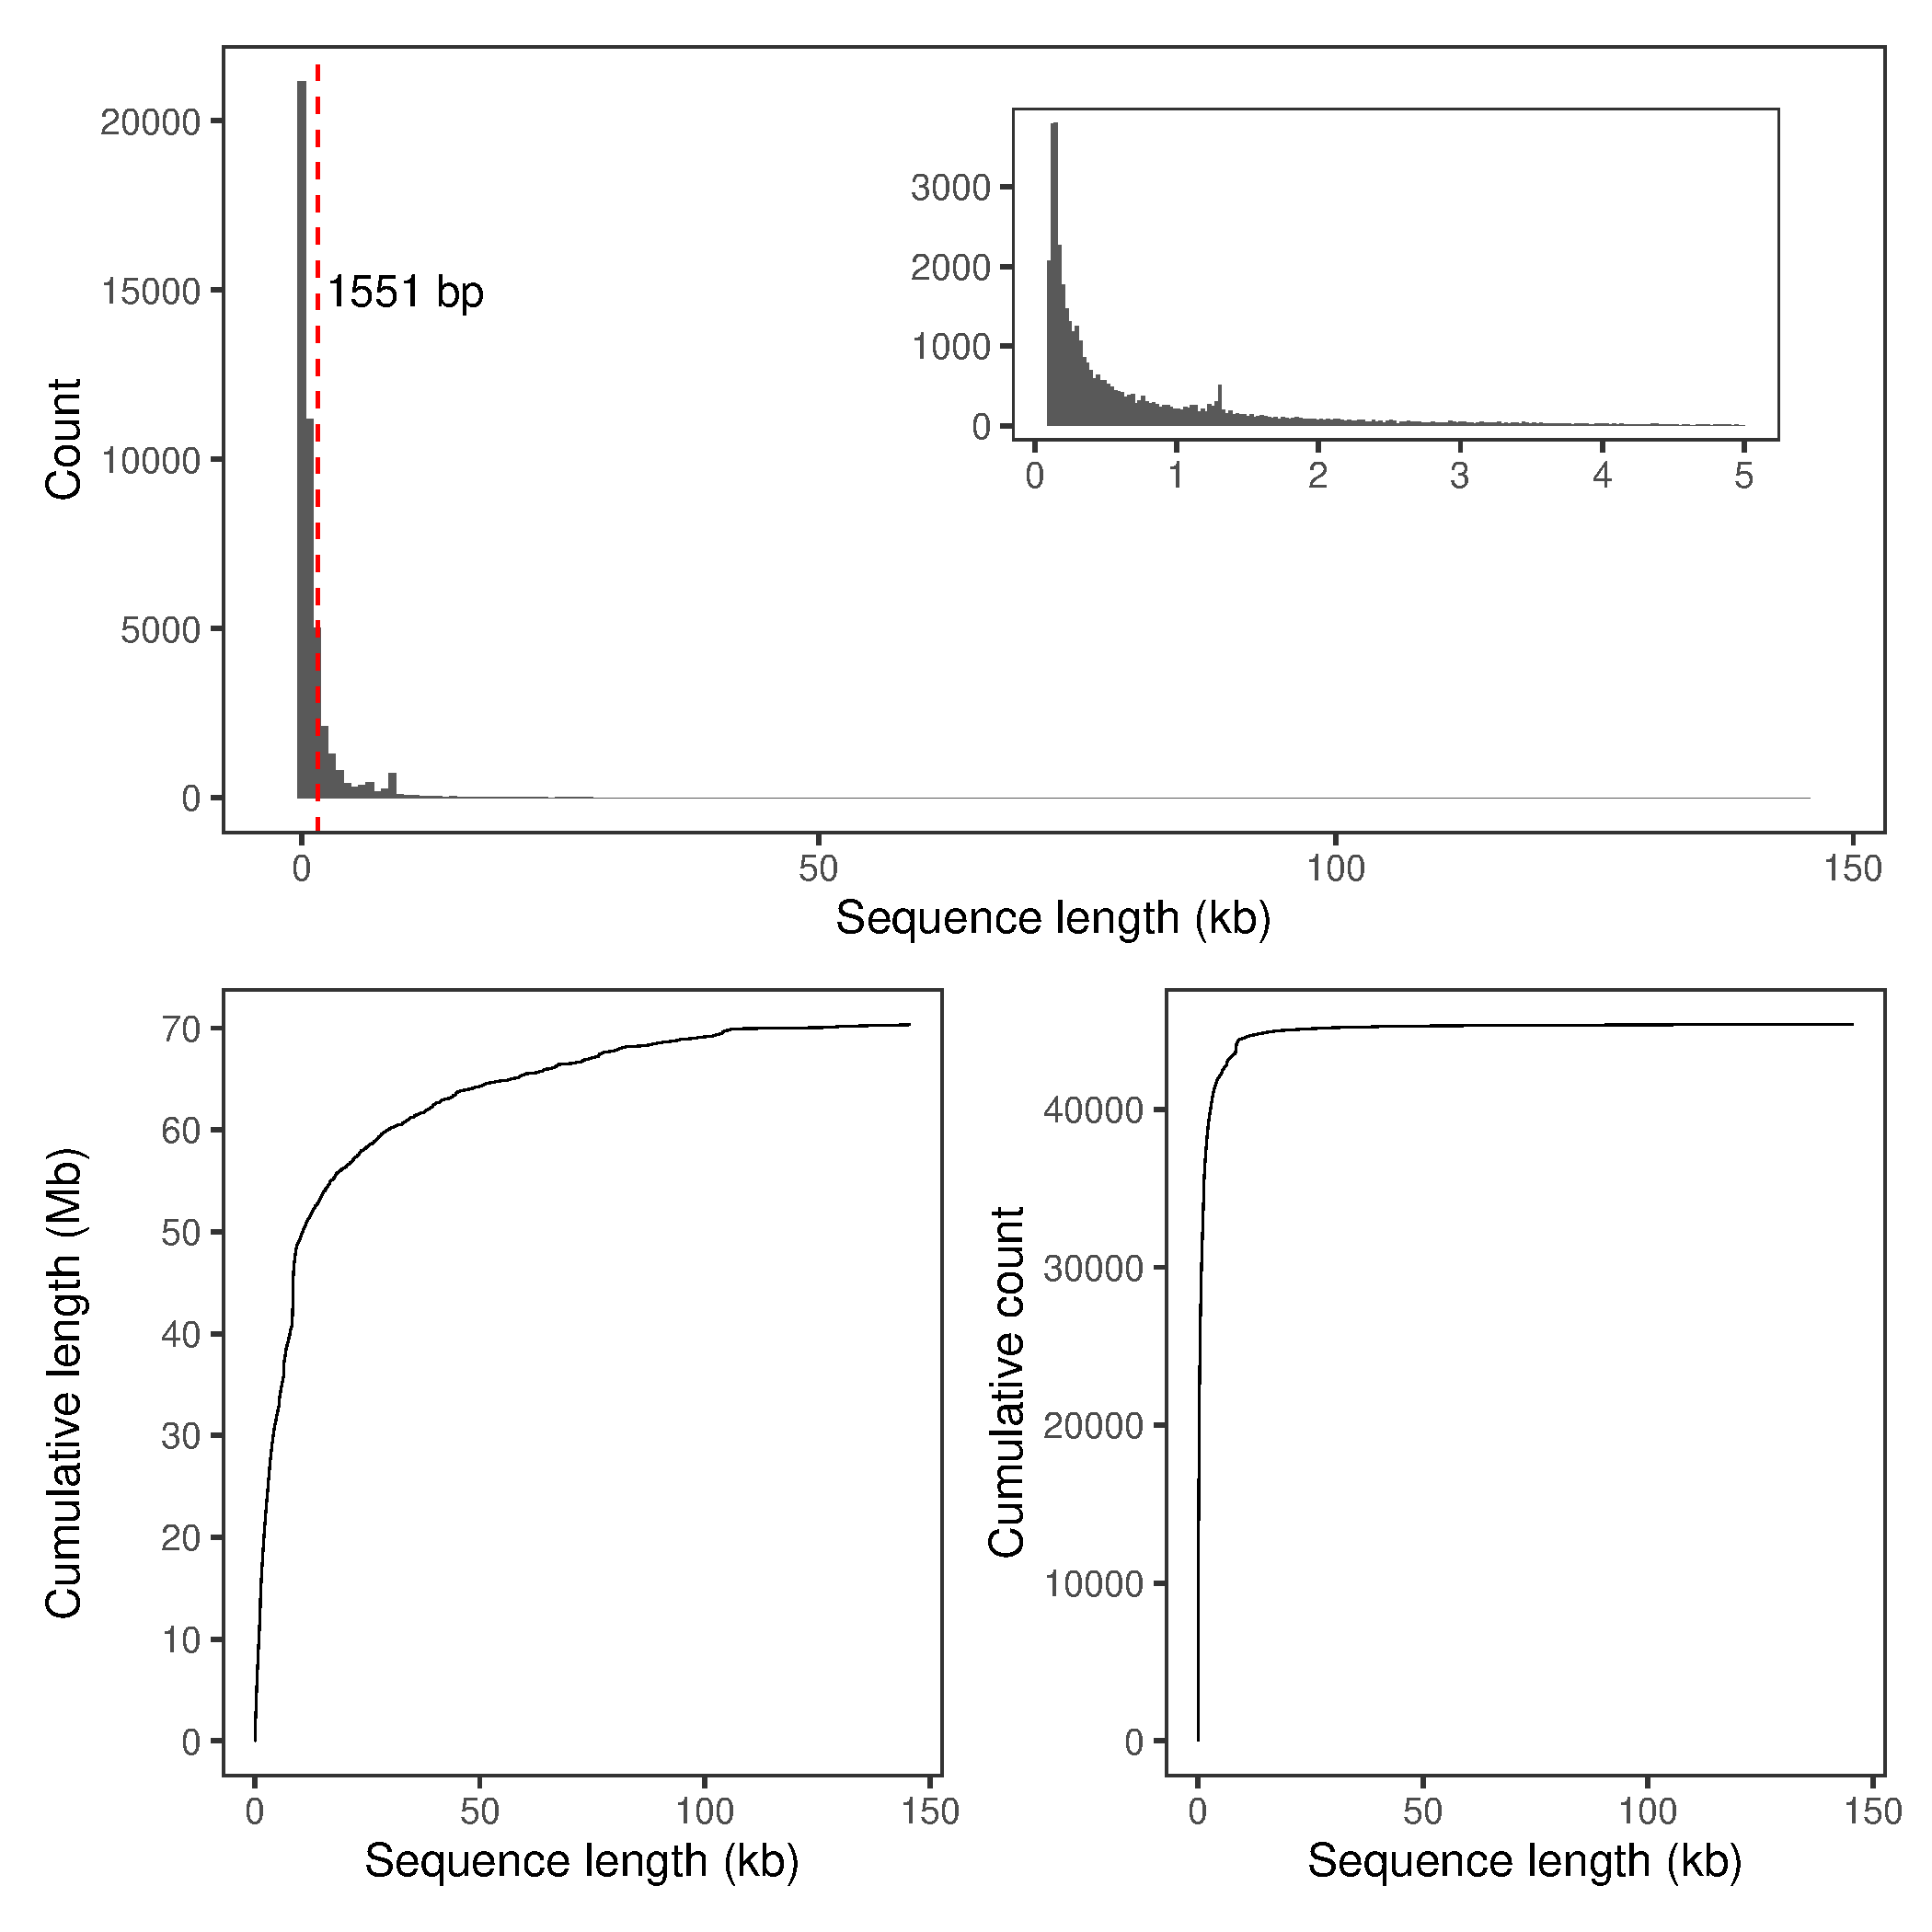
\includegraphics[width=\textwidth]{paper3/supplement/sp46.pdf}
    \caption[Distribution of the nonreference sequences]{\textbf{Length of the non-reference sequences that were added linearly to the ARS-UCD1.2 reference.} \\
    \small{Length distribution of the non-reference alleles (upper panel) and their cumulative length and count (lower panels). The inset in the upper panel displays the distribution of non-reference alleles shorter than 5 kb. The dashed-red line indicates the average length (1551 bp) of the non-reference alleles.}}
    \label{sup_fig:s46}
\end{figure}

\newpage

\begin{figure}[!htb]
    \centering
    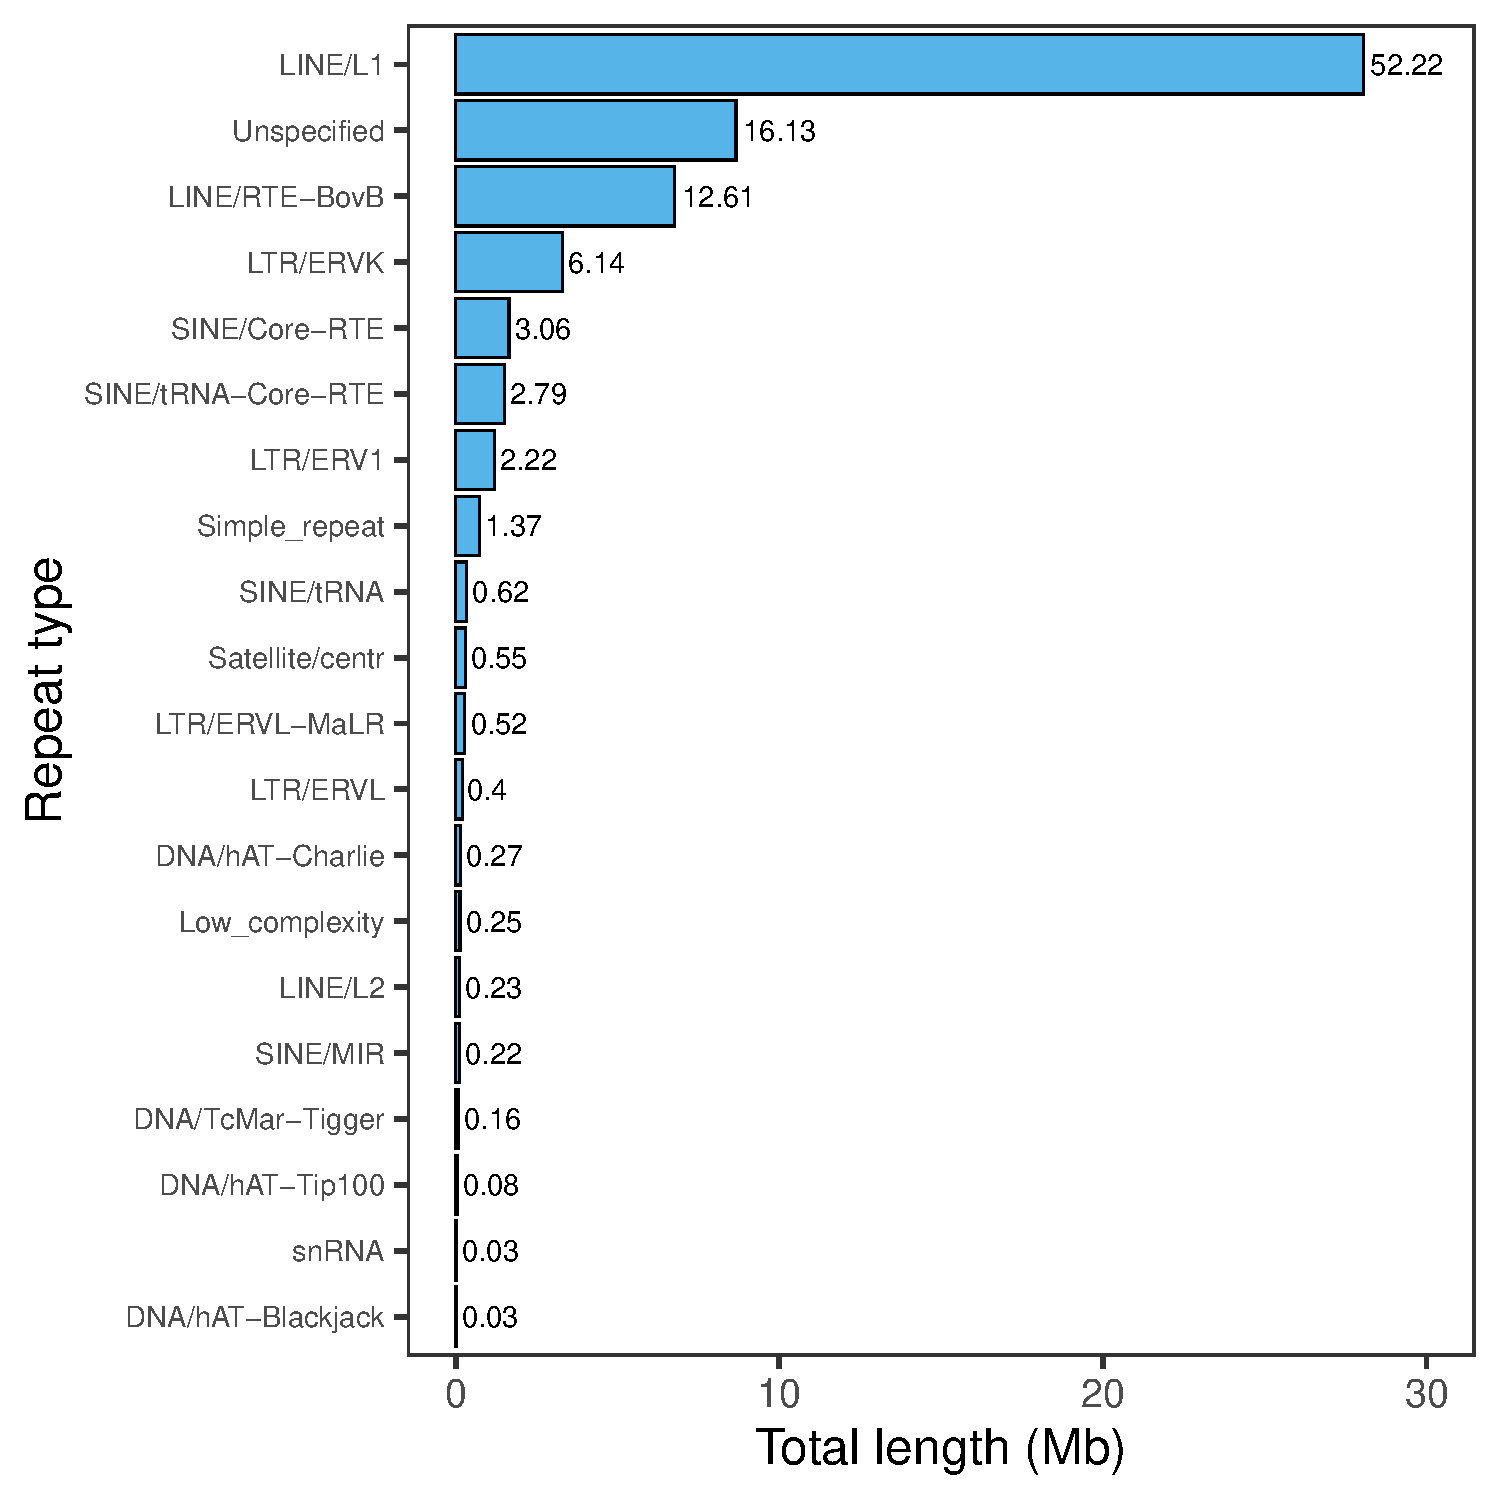
\includegraphics[width=\textwidth]{paper3/supplement/sp47.pdf}
    \caption[Repetitive elements in the pangenome]{\textbf{Prevalence of repetitive elements in the non-reference sequences.}
    \small{The 20 most prevalent repetitive elements account for 99.9\% of the repetitive elements detected in the non-reference sequences. The X-axis indicates the summed sequence length (in Mb) spanned by the repetitive elements, with text labels indicate the proportion (\%) of a repetitive element contributing to the total repeat length. }}
    \label{sup_fig:s47}
\end{figure}

\begin{landscape}
    \begin{figure}[!htb]
        \centering
        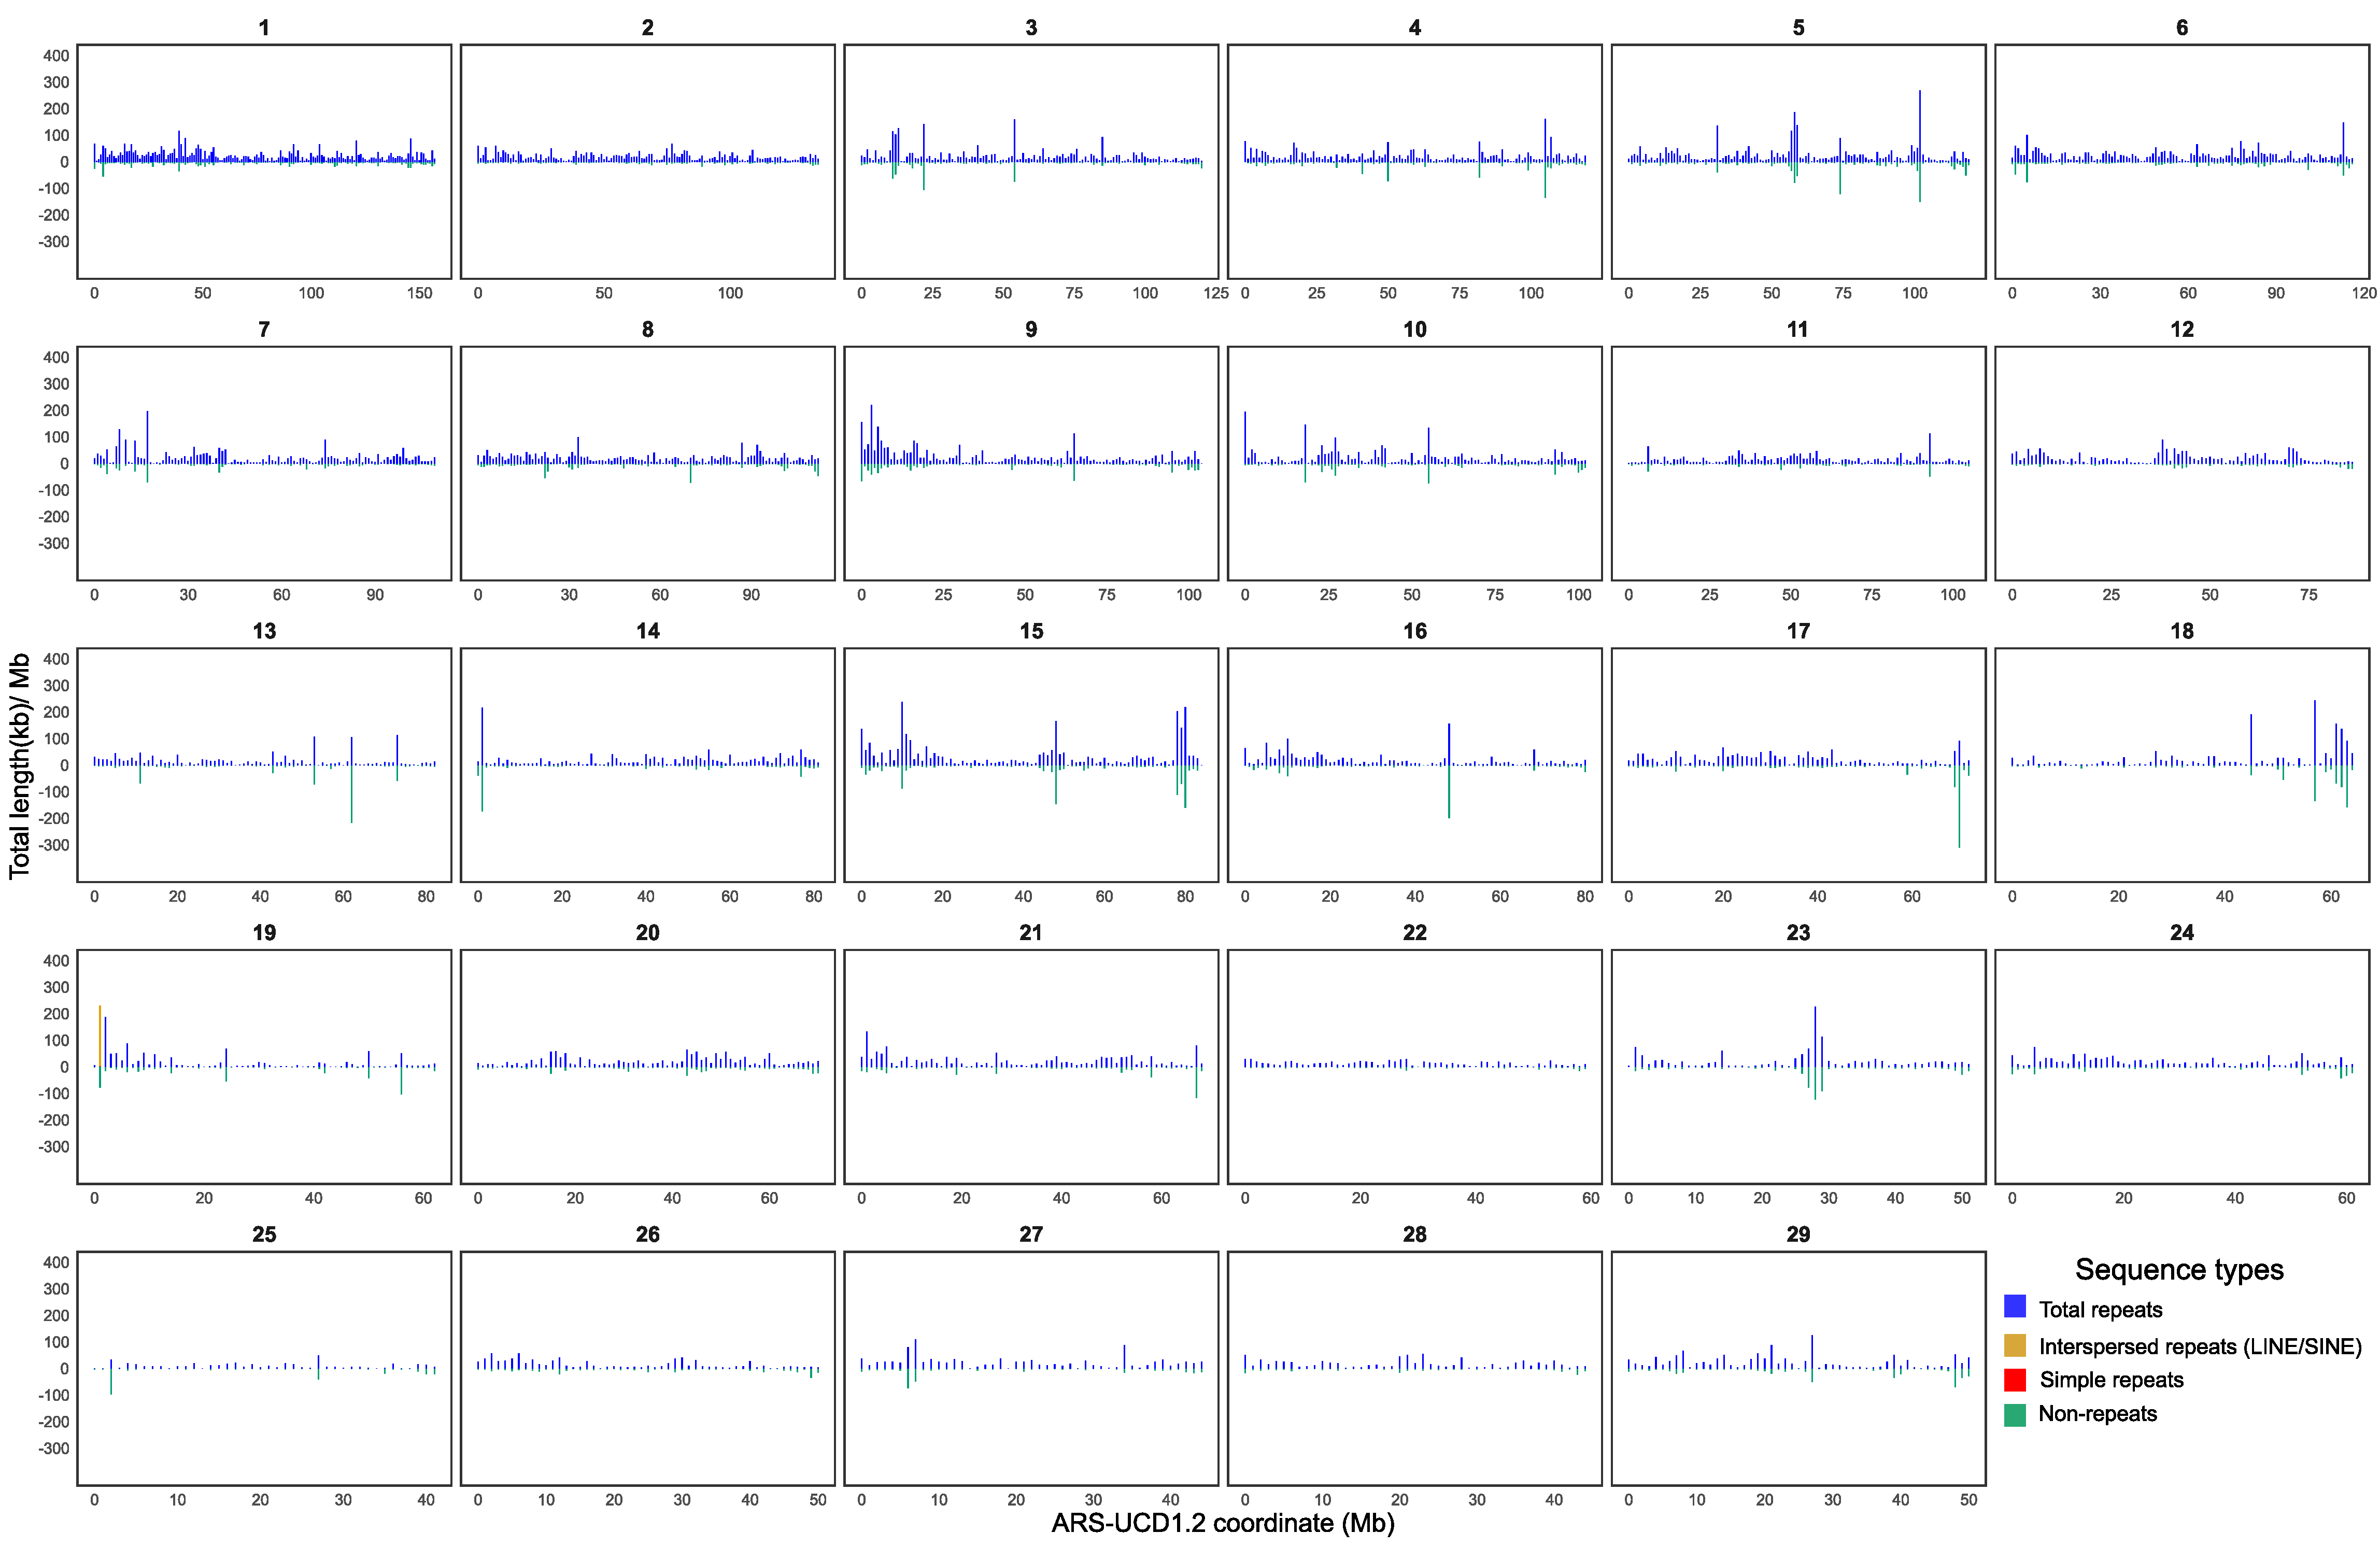
\includegraphics[width=1.5\textwidth]{paper3/supplement/sp48.pdf}
        \caption[Distribution of the repetitive and non-repeat elements]{\textbf{The distribution of repetitive element (interspersed and simple repeats), and non-repetitive elements} \\
        \small{found in non-reference sequences based on the ARS-UCD1.2 coordinate system. To aid visualization, the distribution of non-repetitive segments is mirrored to the negative Y-axis. The numbers above the individual panels are chromosome identifiers.}}
        \label{sup_fig:s48}
    \end{figure}
\end{landscape}

\newpage


\begin{figure}[!htb]
    \centering
    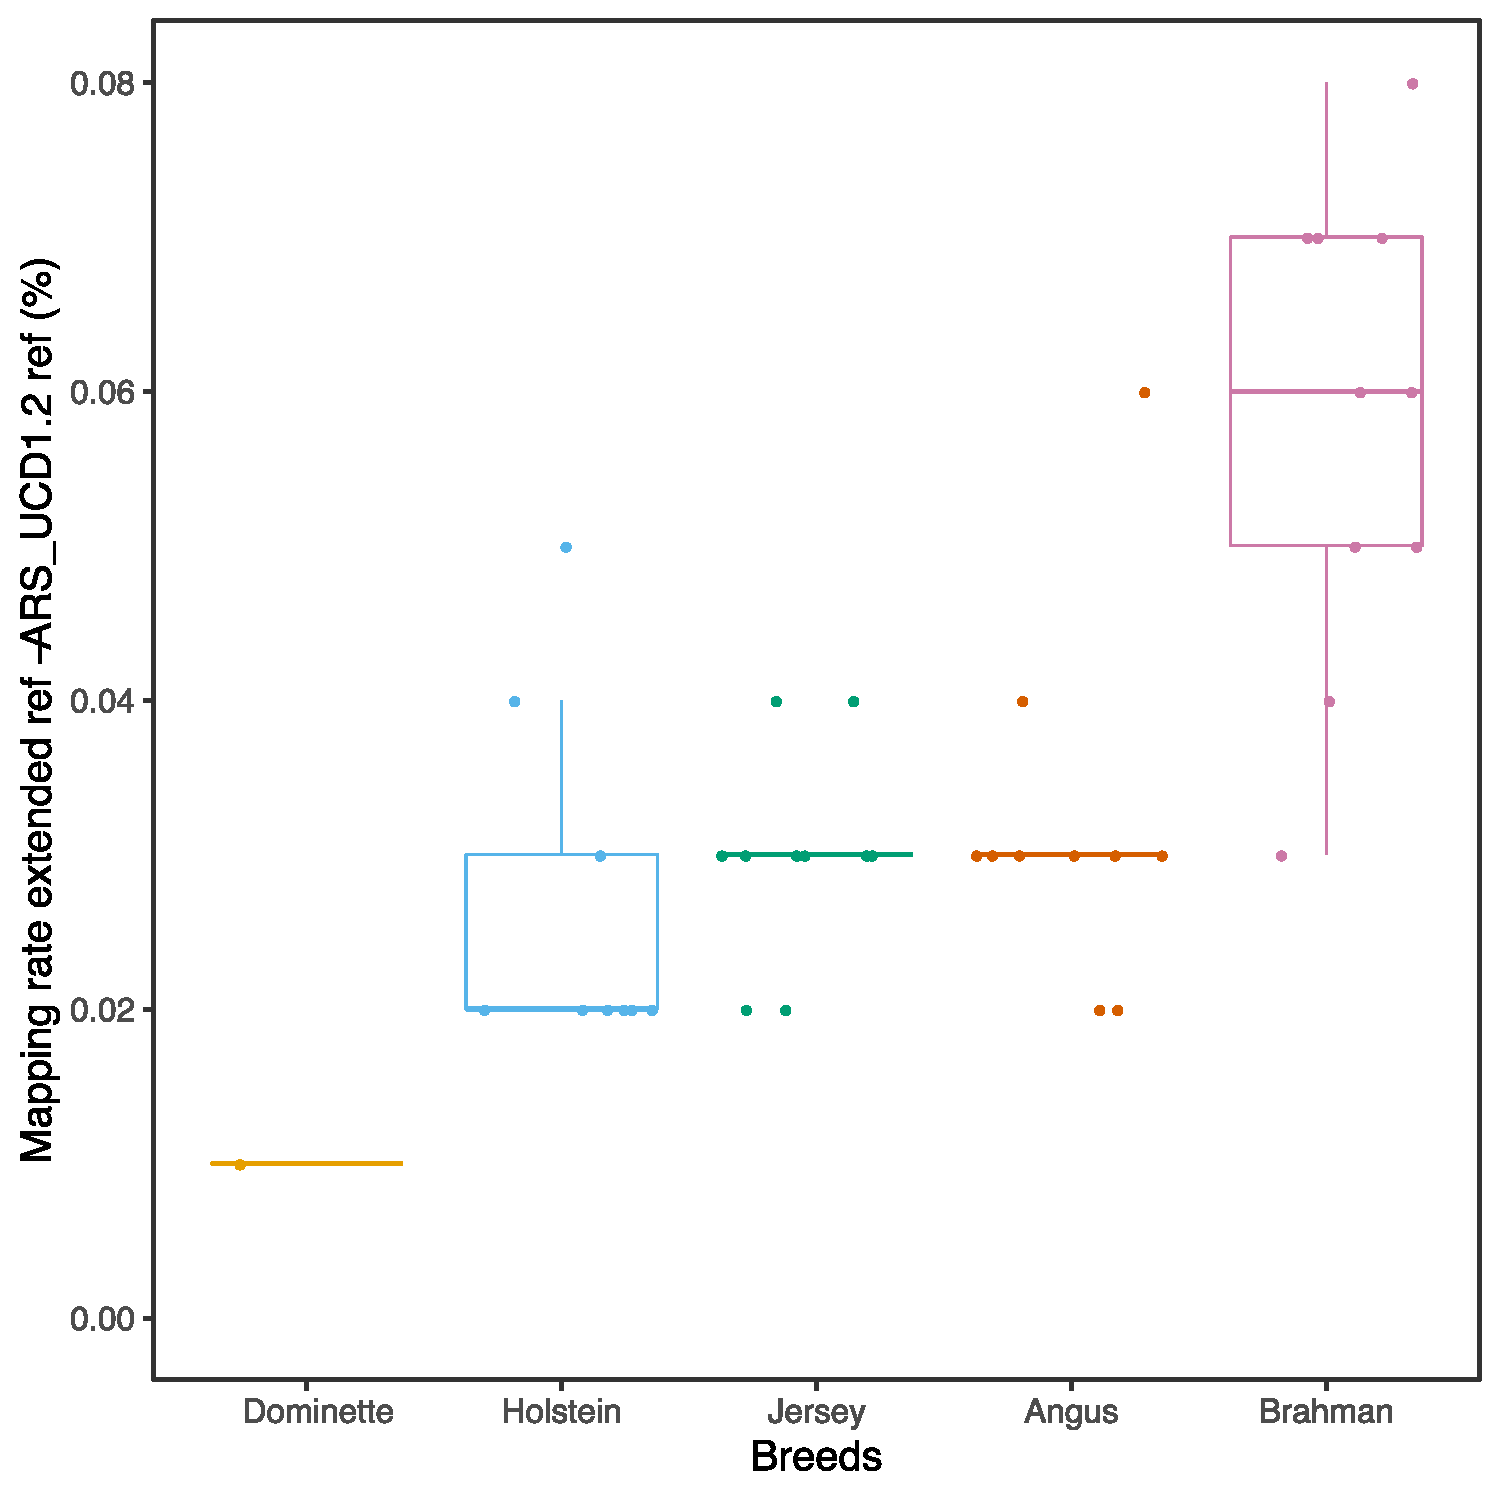
\includegraphics[width=\textwidth]{paper3/supplement/sp49.pdf}
    \caption[Transcriptome mapping improvement in the pangenome]{\textbf{Transcriptome mapping rate improvements in five breeds using the extended reference sequence over ARS-UCD1.2. } \\
    \small{Values along the Y axis represent the difference in mapping rate between the extended and the original ARS-UCD1.2 reference (\%) as reported by HISAT2. Positive values indicate that more reads aligned to the extended than original reference. Dominette is the Hereford animal used to construct ARS-UCD1.2.}}
    \label{sup_fig:s49}
\end{figure}

\newpage

\begin{figure}[!htb]
    \centering
    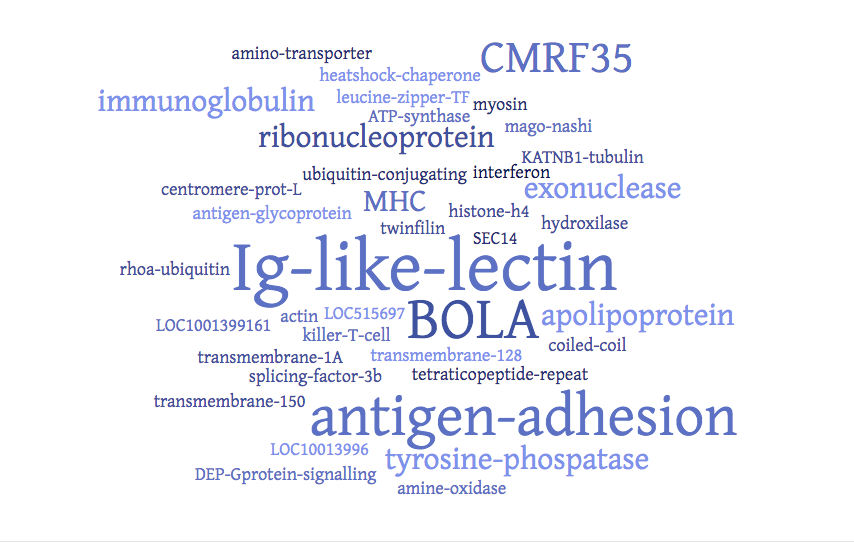
\includegraphics[width=\textwidth]{paper3/supplement/sp410.png}
    \caption[BLAST results of the novel genes]{\textbf{Word cloud of the top blast hits from 142 putatively novel genes assembled from RNA sequencing reads mapping to non-reference sequences.} \\
    \small{The BLAST query was performed against a protein database containing sequences from \emph{Bos} and related species. Word size reflects the frequency of the hits.}}
    \label{sup_fig:s410}
\end{figure}

\newpage

\begin{figure}[!htb]
    \centering
    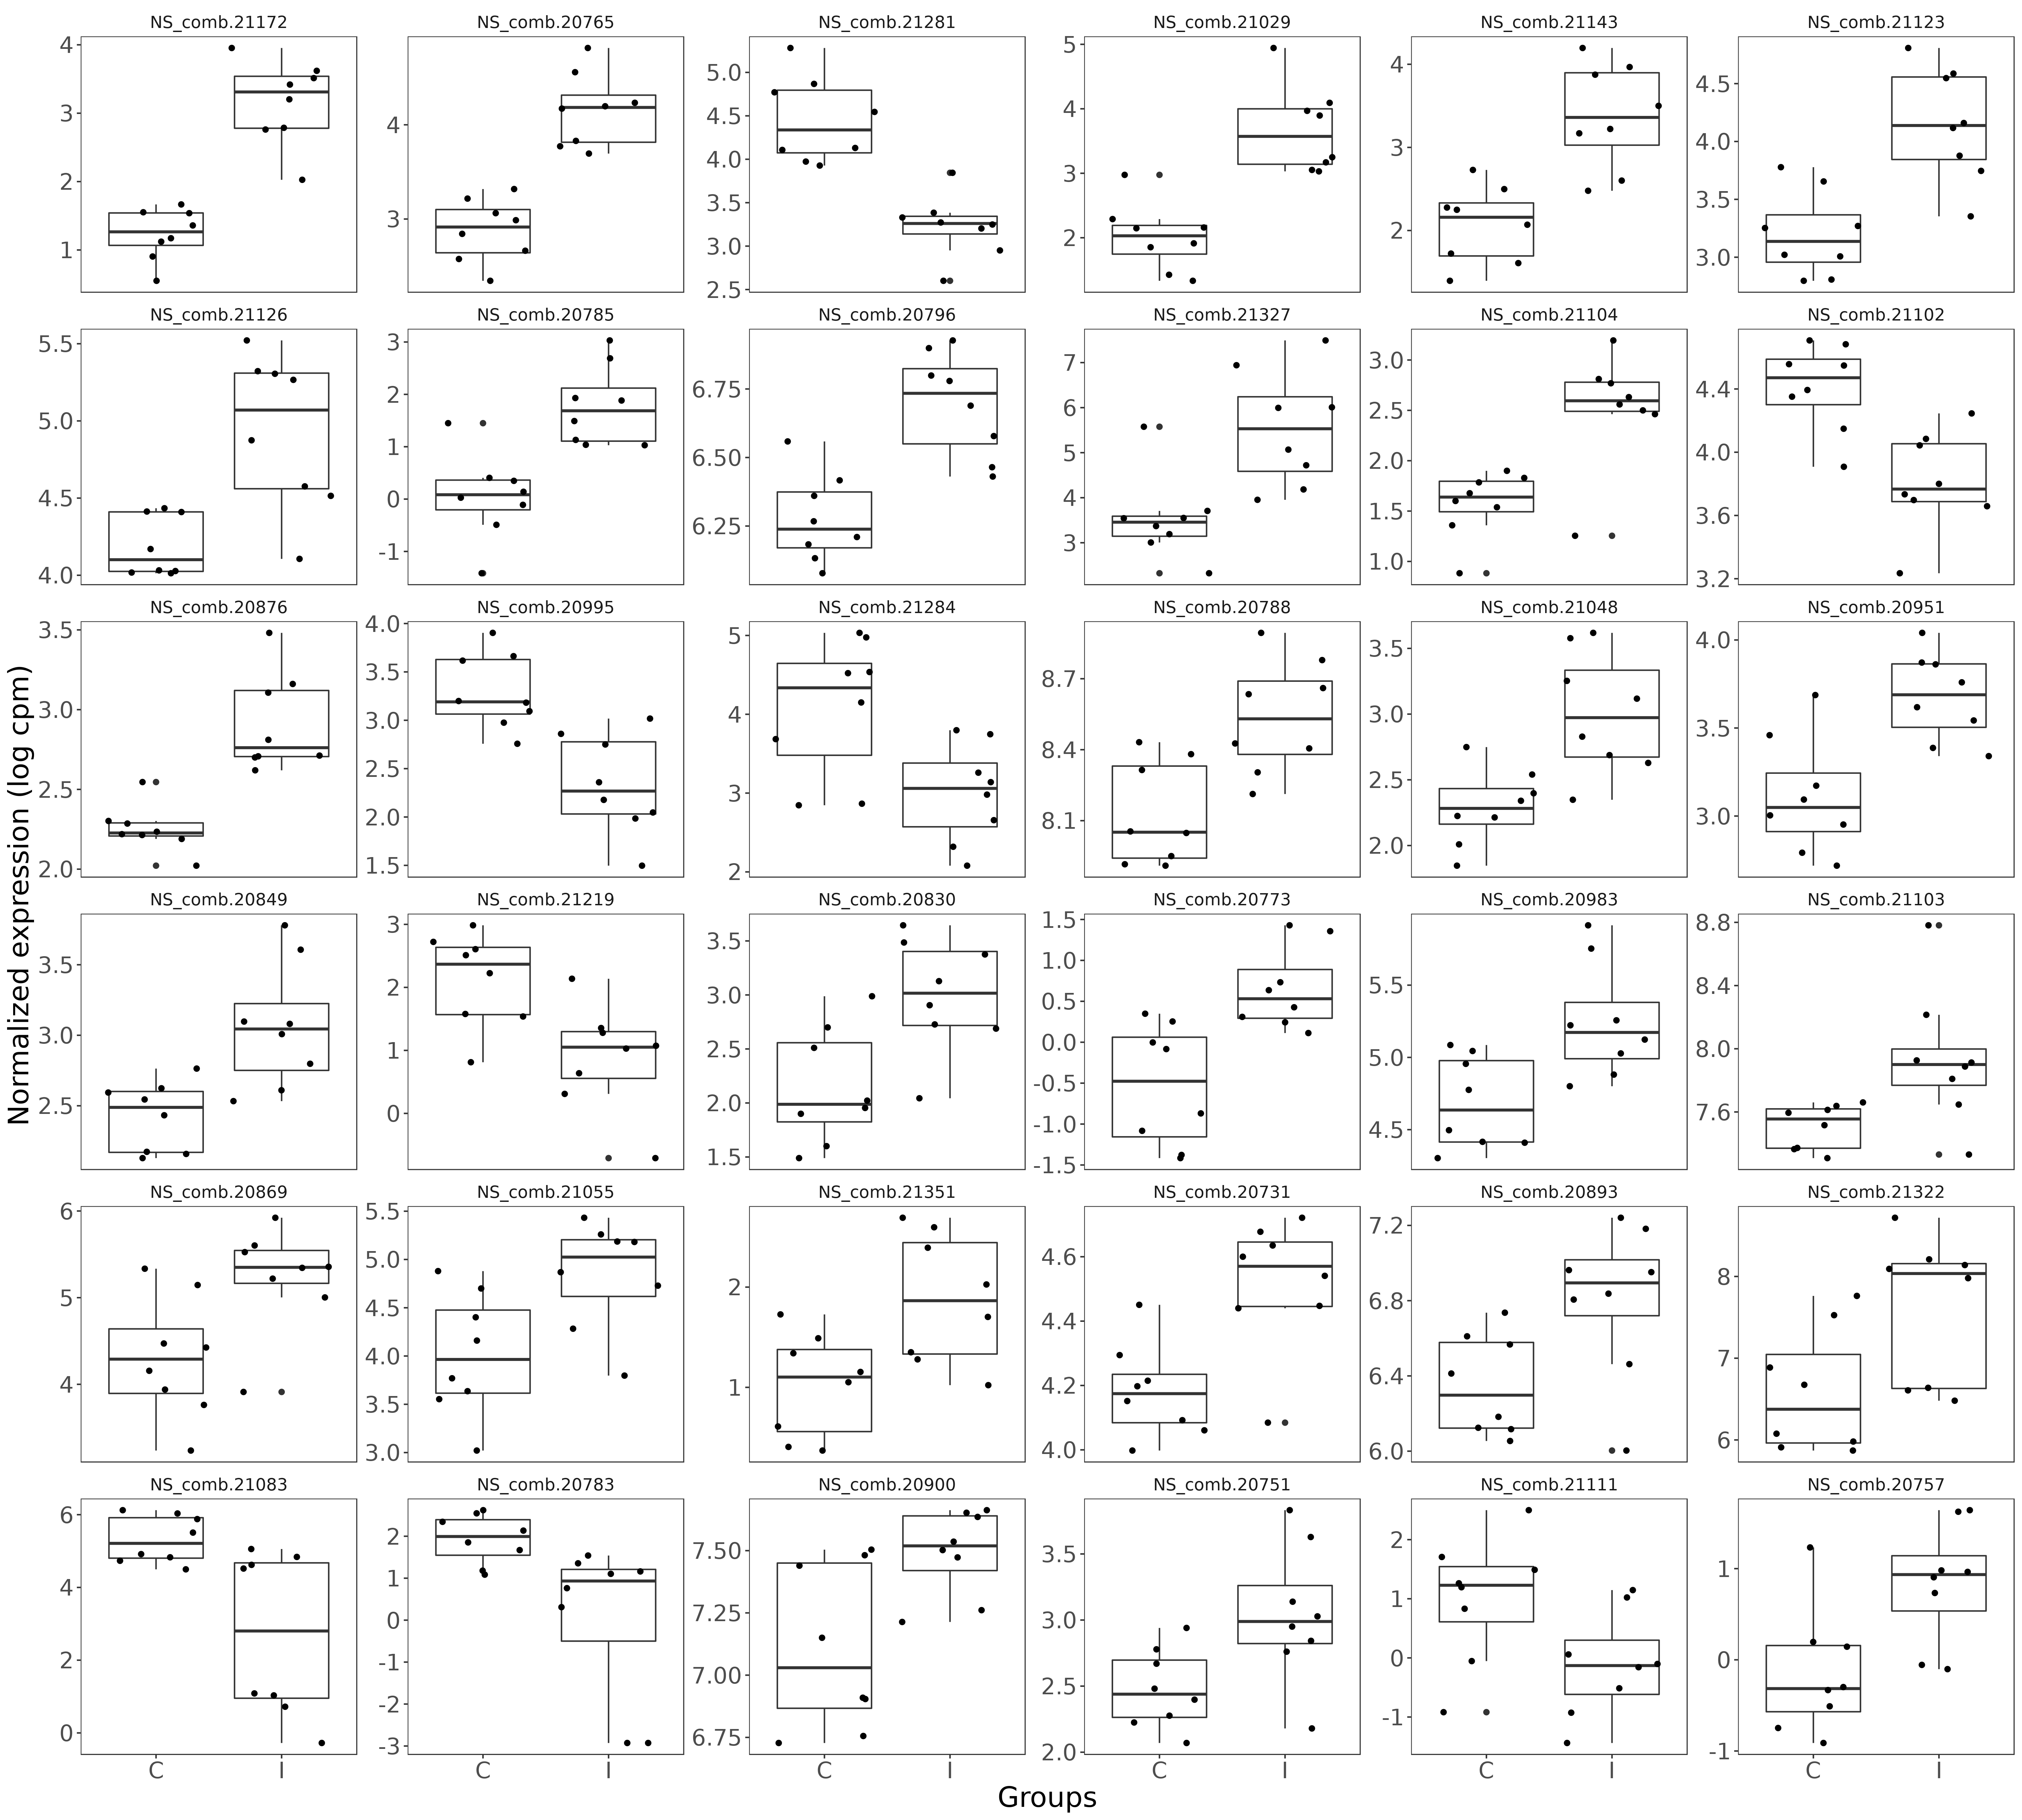
\includegraphics[width=\textwidth]{paper3/supplement/sp411.png}
    \caption[Differential expression of the novel genes]{\textbf{Differential expression of 36 non-reference genes in Mycobacterium bovis-infected cattle.} \\
    \small{Control (C) and \emph{Mycobacterium bovis}-infected (I) cattle are grouped separately for each gene. Y axis indicates the normalized transcript abundance expressed as log$_2$ CPM as reported by EdgeR.}}
    \label{sup_fig:s411}
\end{figure}

\newpage

\begin{figure}[!htb]
    \centering
    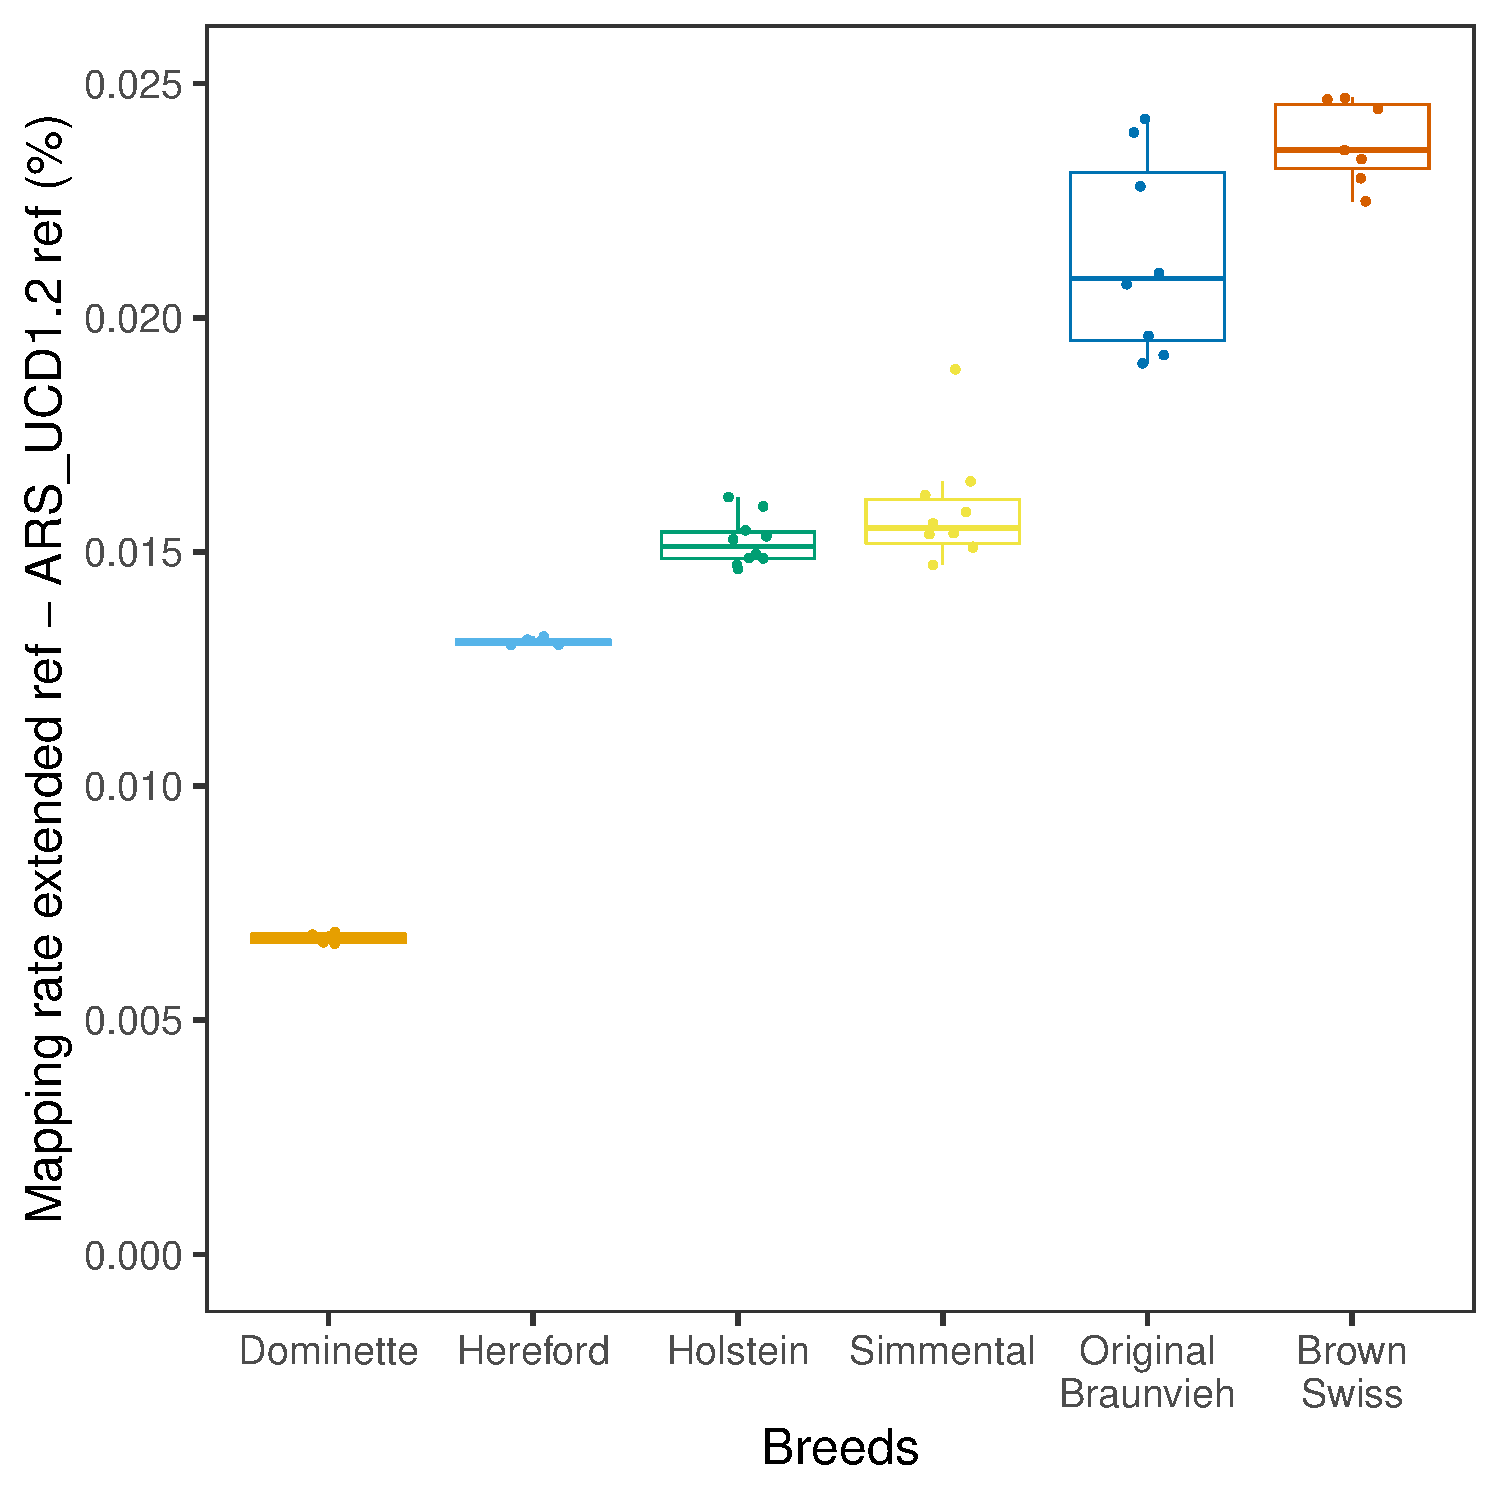
\includegraphics[width=\textwidth]{paper3/supplement/sp412.pdf}
    \caption[WGS mapping improvement to pangenome]{\textbf{Mapping rate of whole-genome short sequencing reads to the extended linear reference genome. } \\
    \small{The Y-axis reflects the difference (in \%) in mapping rate between the extended reference and the original ARS–UCD1.2 reference sequences. Positive values indicate that the mapping rate is higher for samples aligned to the extended than original ARS-UCD1.2 reference sequences. Short sequencing reads of 45 cattle from five breeds were considered. Dominette is a Hereford cattle, but is separated as she is the animal used to construct ARS-UCD1.2.}}
    \label{sup_fig:s412}
\end{figure}

\newpage

\begin{figure}[!htb]
    \centering
    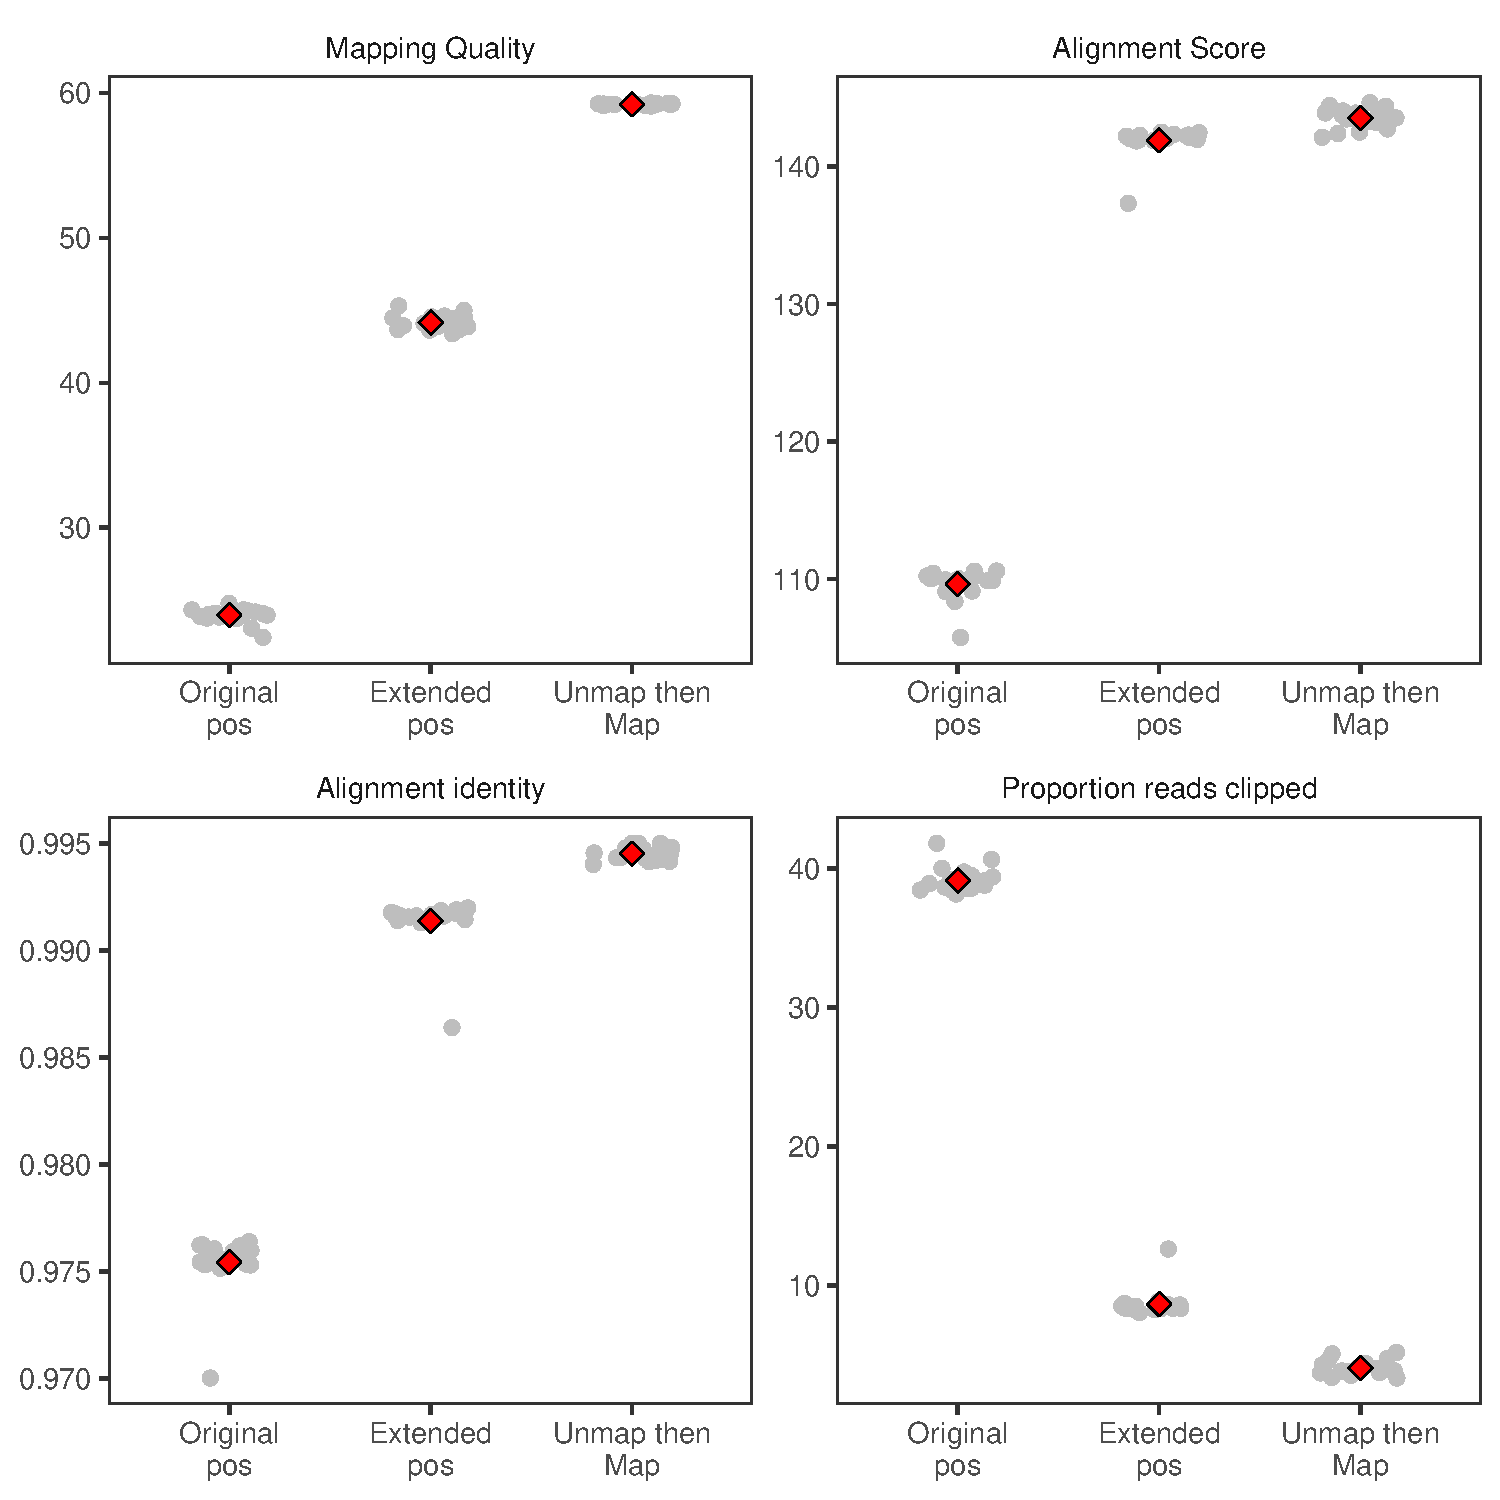
\includegraphics[width=0.7\textwidth]{paper3/supplement/sp413.pdf}
    \caption[Accuracy of read mapping to non-reference sequences]{\textbf{Accuracy of read mapping to non-reference sequences.} \\
    \small{Four mapping statistics (mapping quality, alignment score, alignment identity, proportion of clipped reads) were assessed for short sequencing reads from 45 samples across 5 breeds. First, we consider reads that mapped to autosomal sequences of the ARS-UCD1.2. The mapping statistics of these reads are compared between the ARS-UCD1.2 reference sequence (Original pos) and their mapping position at the novel non-reference sequences of the extended reference genome (Extended pos). Second, we consider reads that were unmapped against the ARS-UCD1.2 reference genome but received a mapping position against the extended reference genome (Unmap then map). Each grey point indicates the average mapping statistics for one DNA sample and red diamond indicates the average across all animals. }}
    \label{sup_fig:s413}
\end{figure}

\newpage

\begin{figure}[!htb]
    \centering
    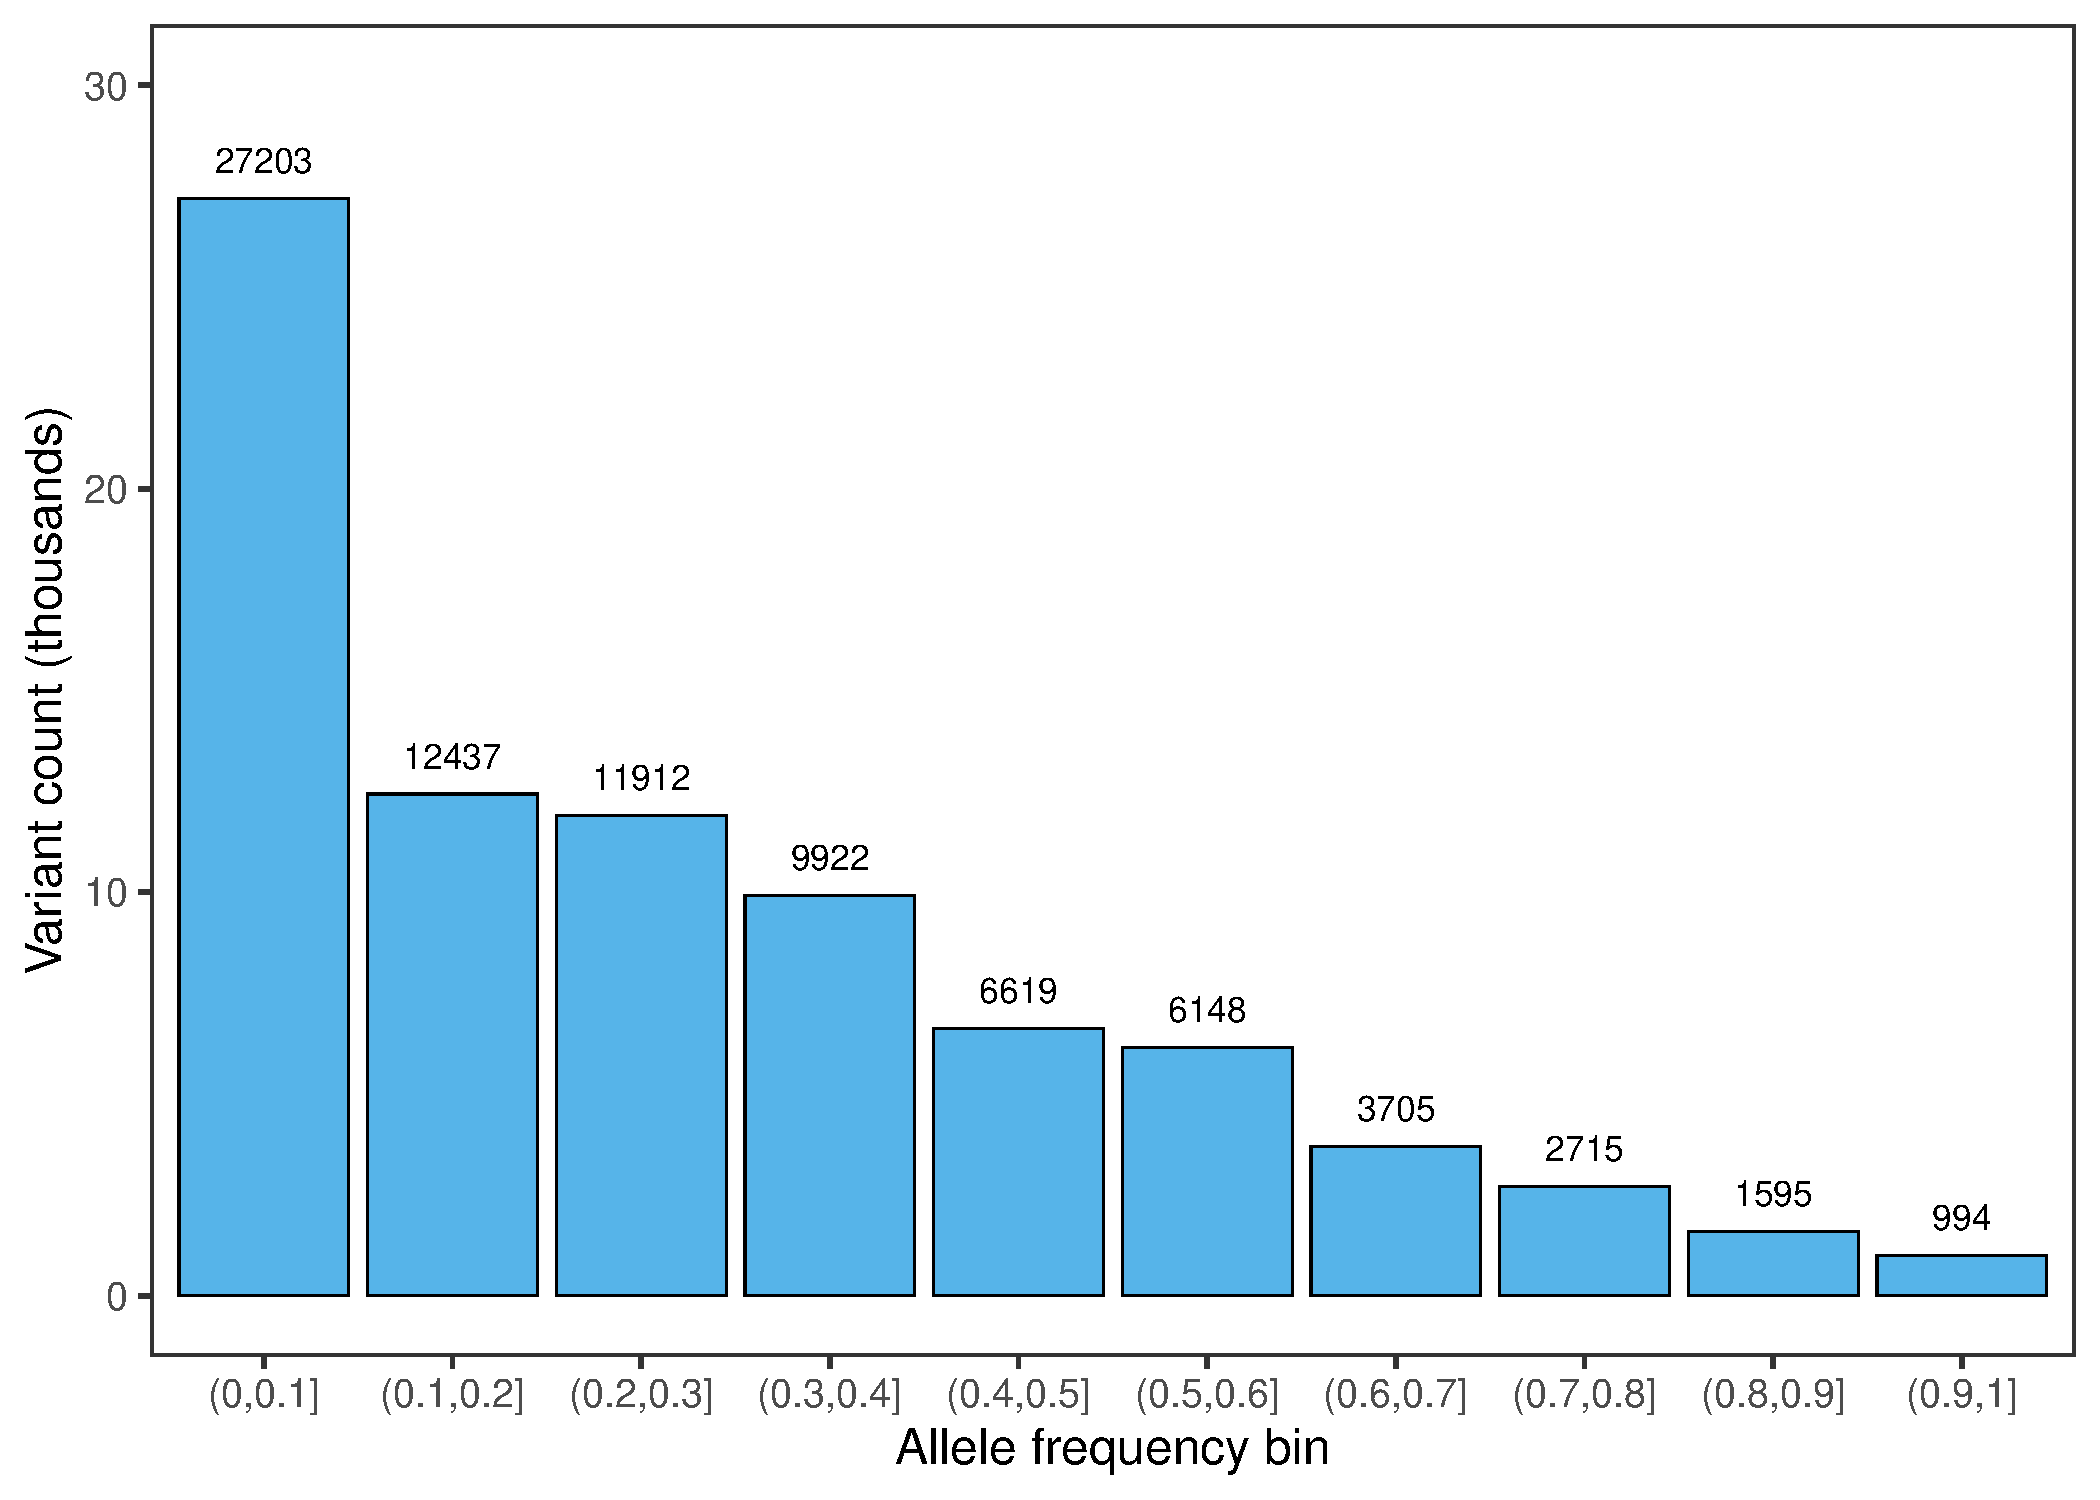
\includegraphics[width=0.8\textwidth]{paper3/supplement/sp414.pdf}
    \caption[Distribuion of variants in non-reference sequences]{\textbf{Alternate allele frequency of 83,250 variants detected from non-reference sequences in 45 samples from 5 breeds.}}
    \label{sup_fig:s414}
\end{figure}

\clearpage
% Supplementary notes


\begin{landscape}
    \begin{table}
        \centering
        \caption[Structural variations extracted from graphs]{\textbf{Different types of structural variations discovered from the multi-assembly graph.}\\
        Variant length is calculated based on the absolute difference between reference and non-reference allele.}
        \bigskip
        \label{sup_tab:s41}
        \begin{tabular}{|l|l|l|l|l|l|l|}
        \hline
        Mutations      & Types        & Count          & Complete type  & Alternate type & Non-ref allele length & Variant length     \\
        \hline
        Insertions     & biallelic    & 35748          & 20432          & 15316          & 40361474              & 37388222           \\
        \hline
        Insertions     & multiallelic & 4621           & 4221           & 400            & 21116534              & 10303720           \\
        \hline
        Deletions      & biallelic    & 28476          & 15377          & 13099          & 2845080               & 28373582           \\
        \hline
        Deletions      & multiallelic & 4661           & 1972           & 2689           & 10130841              & 11727721           \\
        \hline
        \textit{Total} &              & \textit{73506} & \textit{42002} & \textit{31504} & \textit{74453929}     & \textit{87793245}  \\
        \hline
        \end{tabular}
    \end{table}
\end{landscape}

\begin{landscape}
    \begin{table}
        \caption[Gene model predictions]{\textbf{Gene model prediction from repeat masked non-reference sequences.} \\
        \small{Total novel genes denote all gene models (including partial genes) predicted by Augustus. Complete gene models restricted to only full gene models (TSS, start codon, exon, intron, stop-codon present). Transcript, exon, and CDS statistics reported as mean (maximum-minimum) length from the full gene models.}}
        \bigskip
        \bigskip
        \centering
        \label{sup_tab:s42}
        \begin{tabular}{|l|l|}
        \hline
        \textbf{Feature of the gene model}~ & \textbf{Value}                     \\
        \hline
        Total novel genes (distinct SVs)    & 857 (768)                          \\
        \hline
        Complete novel genes (distinct SVs) & 374 (328)                          \\
        \hline
        Transcript length (bp)              & 4742.14 (min: 314; max: 104024)    \\
        \hline
        Exon length (bp)                    & 942.30 (min: 15; max: 6725)        \\
        \hline
        Exon length/gene (bp)               & 2050.89 (min: 314; max: 7762)      \\
        \hline
        Exon count/gene (bp)                & 2.18 (min: 1; max: 20)             \\
        \hline
        CDS length (bp)                     & 396.64 (min: 5; max: 3059)         \\
        \hline
        CDS length/gene (bp)                & 794.34 (min: 199; max: 6280)       \\
        \hline
        protein length (aa)                 & 264.78 (min: 66.33; max: 2093.33)  \\
        \hline
        \end{tabular}
    \end{table}
\end{landscape}


\begin{landscape}
    \begin{table}
        \centering
        \caption[BLAST hits of differentially expressed novel genes]{\textbf{BLASTX hits of the transcripts from differentially expressed non-reference genes} \\
        \small{Log$_2$ FC is the difference in expression between Mycobacterium bovis-infected and non-infected control cattle (e.g., a positive value indicates that expression is higher in infected than control cattle), and Adj FDR is the adjusted false discovery rate determined using the Benjamini-Hochberg correction. }}
        \bigskip
        \bigskip
        \small
        \centering
        \label{sup_tab:s43}
        \begin{tabular}{|l|l|l|l|l|}
        \hline
        \multicolumn{1}{|c|}{\multirow{2}{*}{\textbf{~Hits}}}                  & \multicolumn{2}{c|}{\textbf{Mean (SD) expression in CPM ~}}                    & \multicolumn{1}{c|}{\multirow{2}{*}{\textbf{log$_2$ FC}}} & \multicolumn{1}{c|}{\multirow{2}{*}{\textbf{Adj FDR}}}  \\
        \cline{2-3}
        \multicolumn{1}{|c|}{}                                                 & \multicolumn{1}{c|}{\textbf{Control}} & \multicolumn{1}{c|}{\textbf{Infected}} & \multicolumn{1}{c|}{}                                  & \multicolumn{1}{c|}{}                                   \\
        \hline
        Antigen WC1.1-like                                                     & 2.43 (0.6)                            & 9.54 (3.65)                            & 2.0137                                                 & 1.98E-05                                                \\
        \hline
        Leukocyte immunoglobulin-like receptor subfamily A member 5 isoform X1 & 23.10 (8.30)                          & 9.59 (2.54)                            & -1.2870                                                & 0.0001                                                  \\
        \hline
        PREDICTED: synaptobrevin homolog YKT6                                  & 4.39 (1.36)                           & 11.19 (4.7)                            & 1.3754                                                 & 0.0008                                                  \\
        \hline
        PREDICTED: major vault protein isoform X1                              & 21.70 (3.87)                          & 14.23 (2.88)                           & -0.6140                                                & 0.0040                                                  \\
        \hline
        PREDICTED: heat shock 70 kDa protein 1B                                & 10.18 (2.7)                           & 5.33 (1.94)                            & -0.9511                                                & 0.0041                                                  \\
        \hline
        Elongation factor 1-alpha 1                                            & 282.86 (40.74)                        & 374.22 (63.08)                         & 0.4033                                                 & 0.0093                                                  \\
        \hline
        Heterogeneous nuclear ribonucleoprotein R isoform 2                    & 5.47 (0.94)                           & 8.65 (2.73)                            & 0.6740                                                 & 0.0148                                                  \\
        \hline
        PREDICTED: prothymosin alpha isoform X2                                & 22.02 (10.73                          & 39.85 (12.84                           & 0.8523                                                 & 0.0243                                                  \\
        \hline
        Stathmin isoform a                                                     & 17.56 (7.39)                          & 30.3 (10.17)                           & 0.7823                                                 & 0.0271                                                  \\
        \hline
        Serine/arginine repetitive matrix protein 1 isoform X1                 & 18.3 (1.74)                           & 22.99 (3.29)                           & 0.3293                                                 & 0.0285                                                  \\
        \hline
        BOLA class I histocompatibility antigen, alpha chain BL3-7-like        & 109.32 (61.3)                         & 223.94 (116.59)                        & 1.0387                                                 & 0.0302                                                  \\
        \hline
        Predicted gene, EG665562                                               & 141.66 (31.9)                         & 179.9 (20.92)                          & 0.3440                                                 & 0.0400                                                  \\
        \hline
        PREDICTED: GTP-binding protein SAR1a                                   & 5.71 (1.22)                           & 8.71 (3.28)                            & 0.6231                                                 & 0.0415                                                  \\
        \hline
        \end{tabular}
        \end{table}
\end{landscape}

\begin{landscape}

    \begin{table}
        \centering
        \caption[Mapping comparison between linear genome and the pangenome]{\textbf{Comparison of read mapping accuracy between the extended and ARS-UCD1.2 reference.} \\
        \footnotesize{All metrics were extracted from BAM files using pysam v0.16.0.1 (1). Alignment identity reflects the proportion of bases from an aligned read that match the reference sequence. A read was considered to be clipped if the CIGAR string of the alignment contains tags for either hard- (H) or soft-clipped (S) bases. Supplementary alignments were reported for alignments with an XS tag. Criteria for perfect and unique alignments were based on those reported by Crysnanto and Pausch. Specifically, reads were considered to align perfectly if the edit distance was zero along the entire read (NM:0 tag), and when the CIGAR did not include H or S tags. Unique alignments are reported for reads that either have a single primary alignment or reads that have a secondary alignment (XA tag) but one alignment has a maximum mapping quality score of 60. Reported values are averaged over n=45 samples. Paired one-sided t-tests were conducted with n-1 degrees of freedom. Parameters marked with ‘*’ indicate the null-hypothesis that ARS-UCD1.2 would perform better than the extended reference, while those without marks indicate the reverse. All tests rejected the null hypothesis.
        }}
        \bigskip
        \bigskip
        \centering
        \label{sup_tab:s44}
            \begin{tabular}{|l|l|l|l|l|l|}
            \hline
            \textbf{Parameter}             & \textbf{Extended reference} & \textbf{ARS-UCD1.2} & \textbf{Difference} & \textbf{Stdev} & \textbf{t-statistic \& p-value}  \\
            \hline
            Unmap (\%) *                   & 0.4291                      & 0.4467              & -0.0176             & 0.00461087     & t =-24.12, p = 2.39e-25          \\
            \hline
            Alignment identity 99\% (\%)   & 87.2716                     & 87.1875             & 0.0841              & 0.00433417     & t = 122.72, p = 2.19e-52         \\
            \hline
            Alignment perfect (\%)         & 68.5732                     & 68.4687             & 0.1045              & 0.00667272     & t = 99.04, p = 9.10e-49          \\
            \hline
            Clipped alignment (\%) *       & 2.1335                      & 2.1923              & -0.0588             & 0.00891613     & t = -41.74, p = 2.81e-34         \\
            \hline
            Supplementary alignment (\%) * & 0.2078                      & 0.2219              & -0.0141             & 0.00379671     & t = -23.45, p = 6.69e-25         \\
            \hline
            Unique alignment (\%) *        & 83.2919                     & 83.6016             & -0.3017             & 0.03348539     & t = -58.51, p = 6.50e-40         \\
            \hline
            \end{tabular}
    \end{table}

\end{landscape}

\newpage


\begin{table}[!htb]
    \centering
    \caption[Functional consequences of the non-reference variants]{\textbf{Functional consequences predicted for 83,250 non-reference variants.} \\
    \small{Variant consequences were predicted using VEP (version 91.3) based on a custom annotation file from Augustus. Only the most severe consequence is shown for each variant. }}
    \bigskip
    \bigskip
    \label{sup_tab:s45}
    \begin{tabular}{|l|l|l|l|l|}
    \hline
    \textbf{Variant consequence} & \textbf{SNPs} & \textbf{Indels} & \textbf{All} & \textbf{Proportion (\%)}  \\
    \hline
    splice\_acceptor\_variant    & 4             & 1               & 5            & 0.006                     \\
    \hline
    splice\_donor\_variant       & 2             & 0               & 2            & 0.0024                    \\
    \hline
    frameshift\_variant          & 0             & 26              & 26           & 0.0312                    \\
    \hline
    inframe\_insertion           & 0             & 1               & 1            & 0.0012                    \\
    \hline
    inframe\_deletion            & 0             & 4               & 4            & 0.0048                    \\
    \hline
    splice\_donor\_variant       & 2             & 0               & 2            & 0.0024                    \\
    \hline
    stop\_gained                 & 17            & 0               & 17           & 0.0204                    \\
    \hline
    stop\_lost                   & 1             & 0               & 1            & 0.0012                    \\
    \hline
    start\_lost                  & 3             & 0               & 3            & 0.0036                    \\
    \hline
    missense\_variant            & 700           & 0               & 700          & 0.8408                    \\
    \hline
    splice\_region\_variant      & 45            & 1               & 46           & 0.0553                    \\
    \hline
    synonymous\_variant          & 374           & 0               & 374          & 0.4492                    \\
    \hline
    stop\_retained\_variant      & 1             & 0               & 1            & 0.0012                    \\
    \hline
    coding\_sequence\_variant    & 2             & 0               & 2            & 0.0024                    \\
    \hline
    5\_prime\_UTR\_variant       & 86            & 2               & 88           & 0.1057                    \\
    \hline
    3\_prime\_UTR\_variant       & 1253          & 149             & 1402         & 1.6841                    \\
    \hline
    intron\_variant              & 5809          & 443             & 6252         & 7.5099                    \\
    \hline
    upstream\_gene\_variant      & 2559          & 277             & 2836         & 3.4066                    \\
    \hline
    downstream\_gene\_variant    & 1811          & 179             & 1990         & 2.3904                    \\
    \hline
    intergenic\_variant          & 61040         & 8458            & 69498        & 83.481                    \\
    \hline
    moderate impact              & 701           & 5               & 706          & 0.848                     \\
    \hline
    high impact                  & 27            & 27              & 54           & 0.0649                    \\
    \hline
    \end{tabular}
\end{table}

\newpage

\subsection{}
\label{sup_not:s41}
\textbf{Assembly of the Original Braunvieh (OBV) genome}

\bigskip
The Original Braunvieh primary assembly was generated from PacBio HiFi CCS reads (study accession PRJEB42335 under sample accession SAMEA7759028), generated from subreads with minimum three passes and minimum predicted read quality of 20.  The fastq data contained 86.9 gigabases, corresponding to nearly 30-fold coverage. The CCS reads were filtered by fastp [0.21.0] \citep{chen2018fastp} with minimum average quality of Q20 and minimum read length of 1kb, with 99.99\% of the data passing these thresholds. Hifiasm [v0.13-r308] \citep{cheng2021haplotype} was then used to generate the assembly from the reads using the additional parameters “-r 4 -a 5 -n 5” on a computing cluster. Hifiasm yields the primary contigs in the GFA format, which were then converted using gfatools [0.4-r196-dirty] into a fasta sequence representation. These contigs were then scaffolded using RagTag [v1.0.1] \citep{alonge2019ragoo} to the ARS-UCD1.2 reference, with custom parameters “--mm2-params "-c -x asm5" -r -m 1000000”.

\bigskip

The contigs were validated for contiguity, completeness, and correctness by multiple independent tools, available in a Snakemake [5.26.1] \citep{koster2012snakemake} pipeline online at \url{https://github.com/AnimalGenomicsETH/bovine-assembly}. Basic contiguity was determined through the asmstat command of paftools \citep{li2018minimap2}. Similarly, the NGA50 value was determined through mapping the contigs to the ARS-UCD1.2 reference, and subsequently considering the length of alignment blocks again with asmstat. These values are described in \hyperlink{Table SN41}{Table SN41}.

\bigskip

\textbf{\hypertarget{Table SN41}{Table SN41}: Contiguity metrics of the primary Original Braunvieh assembly.} \\
\footnotesize{Size refers to the total number of bases in the chromosomes and unplaced contigs. NG50 was calculated for both the contig set and the scaffolded assembly with the expected genome size taken from the ARS-UCD1.2 reference. Similarly, NGA50 is the NG50 value for aligned blocks of the assembly to the ARS-UCD1.2 reference.}
\begin{center}
    \begin{tabular}{|c|c|c|c|c|c|c|}
    \hline
    ~        & Size   & Contig NG50 & NGA50 & Scaffold NG50 & L50 & Contigs  \\
    \hline
    assembly & 3.17gb & 86.0        & 68.9  & 96.3          & 15  & 765      \\
    \hline
    \end{tabular}
\end{center}

\normalsize

Completeness of the assembly was determined through two independent approaches, BUSCO (8) and the asmgene command of paftools. The former relies on the OrthoDB datasets, specifically version 10 of the cetartiodactyla lineage. The latter uses cDNA libraries of annotated gene sequences from the ARS-UCD1.2 reference available from Ensembl. Both methods report a high completeness (>96\%) with respect to predicted gene content, as shown in \hyperlink{Table SN42}{Table SN42}.

\newpage

\textbf{\hypertarget{Table SN42}{Table SN42}: Predicted single-copy gene completeness of the primary Original Braunvieh assembly.} \\
\footnotesize{Single-copy refers to genes that were correctly present once in assembly, while duplicates are genes which appeared more than expected. Fragmented genes are those which are only partially mapped, or fully mapped but split into multiple pieces. Missing genes are either not found or mapped below 10\% of the expected gene. }
\begin{center}
    \centering
    \begin{tabular}{|l|l|l|l|l|l|}
    \hline
    ~       & Single copy & duplicates & fragmented & missing & total  \\
    \hline
    Busco   & 12533       & 283        & 166        & 353     & 13335  \\
    \hline
    asmgene & 18503       & 166        & 68         & 136     & 18873  \\
    \hline
\end{tabular}
\end{center}

\normalsize
\bigskip

Correctness was likewise determined by two k-mer based approaches, yak [r58] \citep{cheng2021haplotype} and Merqury \citep{rhie2020merqury}. Yak uses an approximate hash-table approach, while Merqury can be run in an exact mode. Both used short read sequences (2x150 bp) from the primary animal, which importantly were not used in generating the assembly, allowing for an independent evaluation. In addition, short read sequences from both parents enabled a quantification of the switch error rate. Only yak provided an estimate of the Hamming error rate, while only Merqury provides phased block statistics. An overview of these statistics is shown in \hyperlink{Table SN43}{Table SN43}.

\bigskip

\textbf{\hypertarget{Table SN43}{Table SN43}: K-mer based, reference-free validation of the primary Original Braunvieh assembly.} \\
\footnotesize{Assembly quality value (QV) is given as a Phred quality score. Completeness estimates how many k-mers present in the short reads are found in the assembly contigs. The switch error rate is calculated differently by yak and Merqury, measuring the percent of wrongly phased adjacent SNPs in yak while in Merqury it measures the percent of wrongly phased haplotype-specific k-mers (“hap-mers”). There are more than 100 phase switches within a 20kb window (long-range switch). The Hamming error is the percent of SNP sites that are phased wrongly. The phase block statistic is the N50 after contigs have been broken at long-range switches, defined as more than 100 wrongly phased hap-mers per 20kb window.}

\begin{center}
    \centering
    \begin{tabular}{|l|l|l|l|l|l|}
    \hline
    ~       & QV    & Completeness & Switch error & Hamming error & Phased N50  \\
    \hline
    Yak     & 48.76 & 100          & 0.012        & 0.37          & -           \\
    \hline
    Merqury & 50.85 & 93.46        & 0.08         & -             & 2.5 mb      \\
    \hline
    \end{tabular}
\end{center}

\normalsize
\bigskip

Furthermore, the assembly was validated by comparing structural variants called by pbsv [2.4.0] between the reads and the ARS-UCD1.2 reference and those called by mumandco [v2.4.2] \citep{o2020mum} between the assembly and the reference. There was good concordance between these approaches, for example an 8kb inversion identified in chromosome six of the assembly matched an 8kb inversion predicted by the read mapping.

\bigskip

The repeat content of the assembly was also in line with expectations, with approximately 48\% of the assembly consisting of repeat elements or low complexity regions according to RepeatMasker version 4.1.1 \citep{Smit2015} using the Repbase repeat database (release 20181026) \citep{bao2015repbase}. Several bovine-specific repeats were identified, along with telomeric or centromeric sequences not present in the existing ARS-UCD1.2 reference, indicating that several contigs are approaching chromosomal-scale and completeness.

\newpage

\subsection{}
\label{sup_not:s42}
\textbf{Determination of the core and flexible parts of the pangenome graph}
\bigskip

To investigate if the order of assemblies used to establish the multi-assembly graph impacts the core and flexible parts, we added the assemblies randomly to the graph. Core genome represents bases shared across all assemblies in the graph, while flexible genome represents number of bases that are variable across assemblies (i.e., not found in all assemblies) \citep{golicz2020pangenomics}. The pangenome increased gradually with the number of assemblies added, driven by an increase in the flexible genome. The core genome size decreased from 2480 Mb to 2400 Mb in the full graph (\hyperlink{Figure SN41}{Figure SN41}), indicating that more genomic segments are variable across bovine species as we add more assemblies into the graph.
\bigskip

\begin{figure}[!htb]
    \centering
    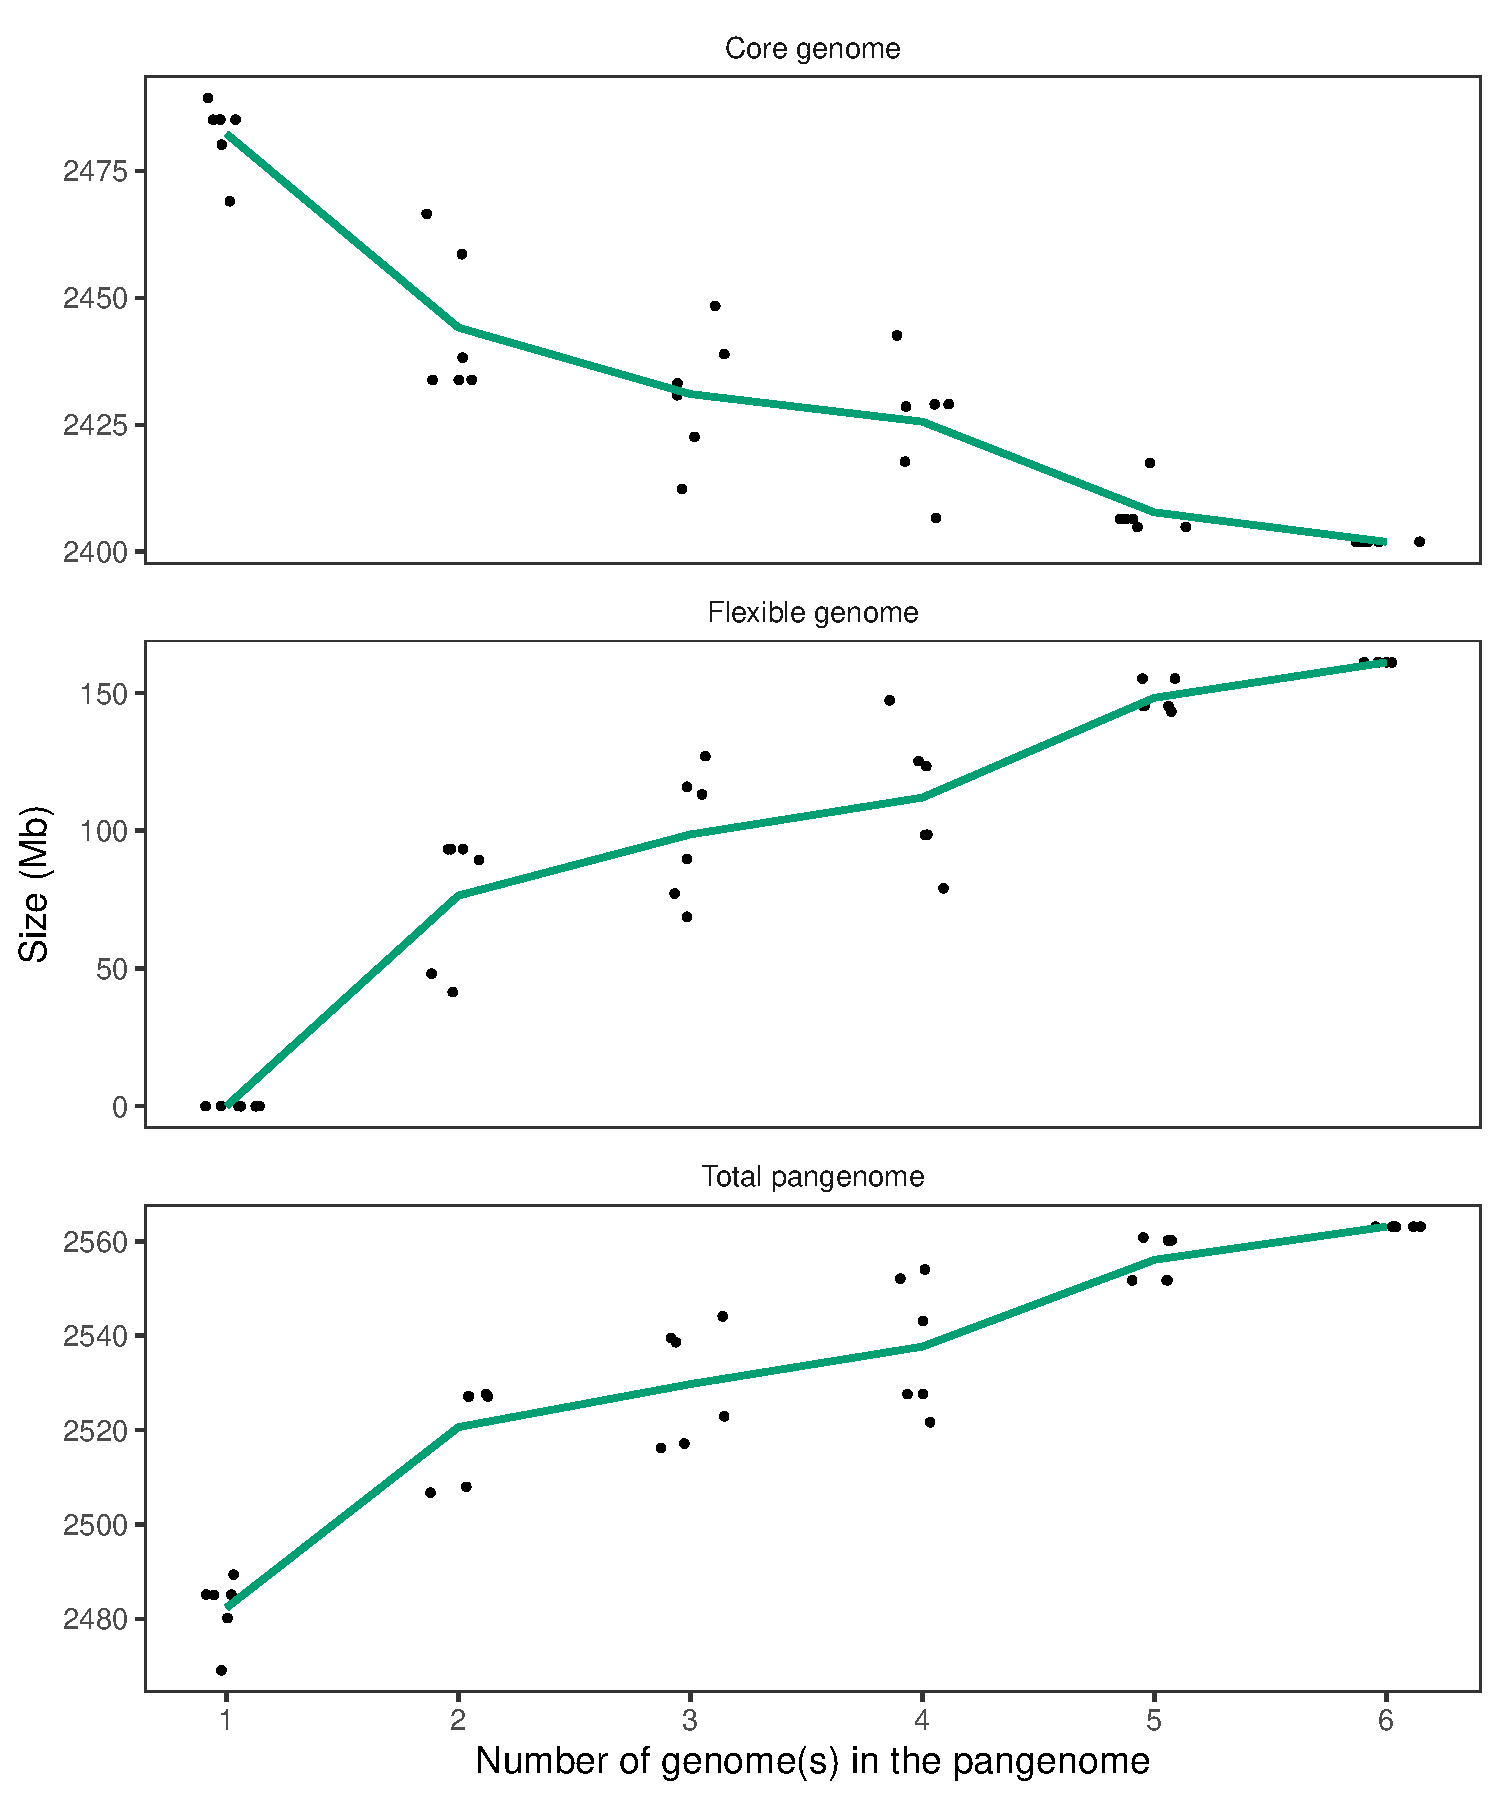
\includegraphics[width=0.7\textwidth]{paper3/supplement/sp415.pdf}
    \caption*{\textbf{\hypertarget{Figure SN41}{Figure SN41}: Profile of the multi-assembly graph with an increasing number of genomes integrated into the graph.} \\
    \footnotesize{We varied the order and number of genomes added to the graphs, and calculated the number of bases in the pangenome, number of bases that are shared across all assemblies in the graph (core genome), and the number of bases that are variable across assemblies (i.e., not found in all assemblies, flexible genome). Points and lines indicate individual and average values.}}
\end{figure}

\bigskip
Next, we investigated the profile of a multi-assembly graph that gradually increases in complexity. We built taurine-only graphs that contained either all or all but one taurine assemblies, a TauInd (four taurine and one indicine), and a full graph (four taurine, one indicine, and yak). The profile of the pangenome changed markedly as more distant assemblies were added to the graph. For example, the flexible part declined substantially from 6.10\% in the full graph to 3.83\% and 2.76\% for the TauInd and taurine-only graph, respectively. However, when an individual taurine assembly is removed from the taurine-only graphs, the size of the flexible part changes only slightly (hyperlink{Figure SN42}{Figure SN42}).

\bigskip
\begin{figure}[!htb]
    \centering
    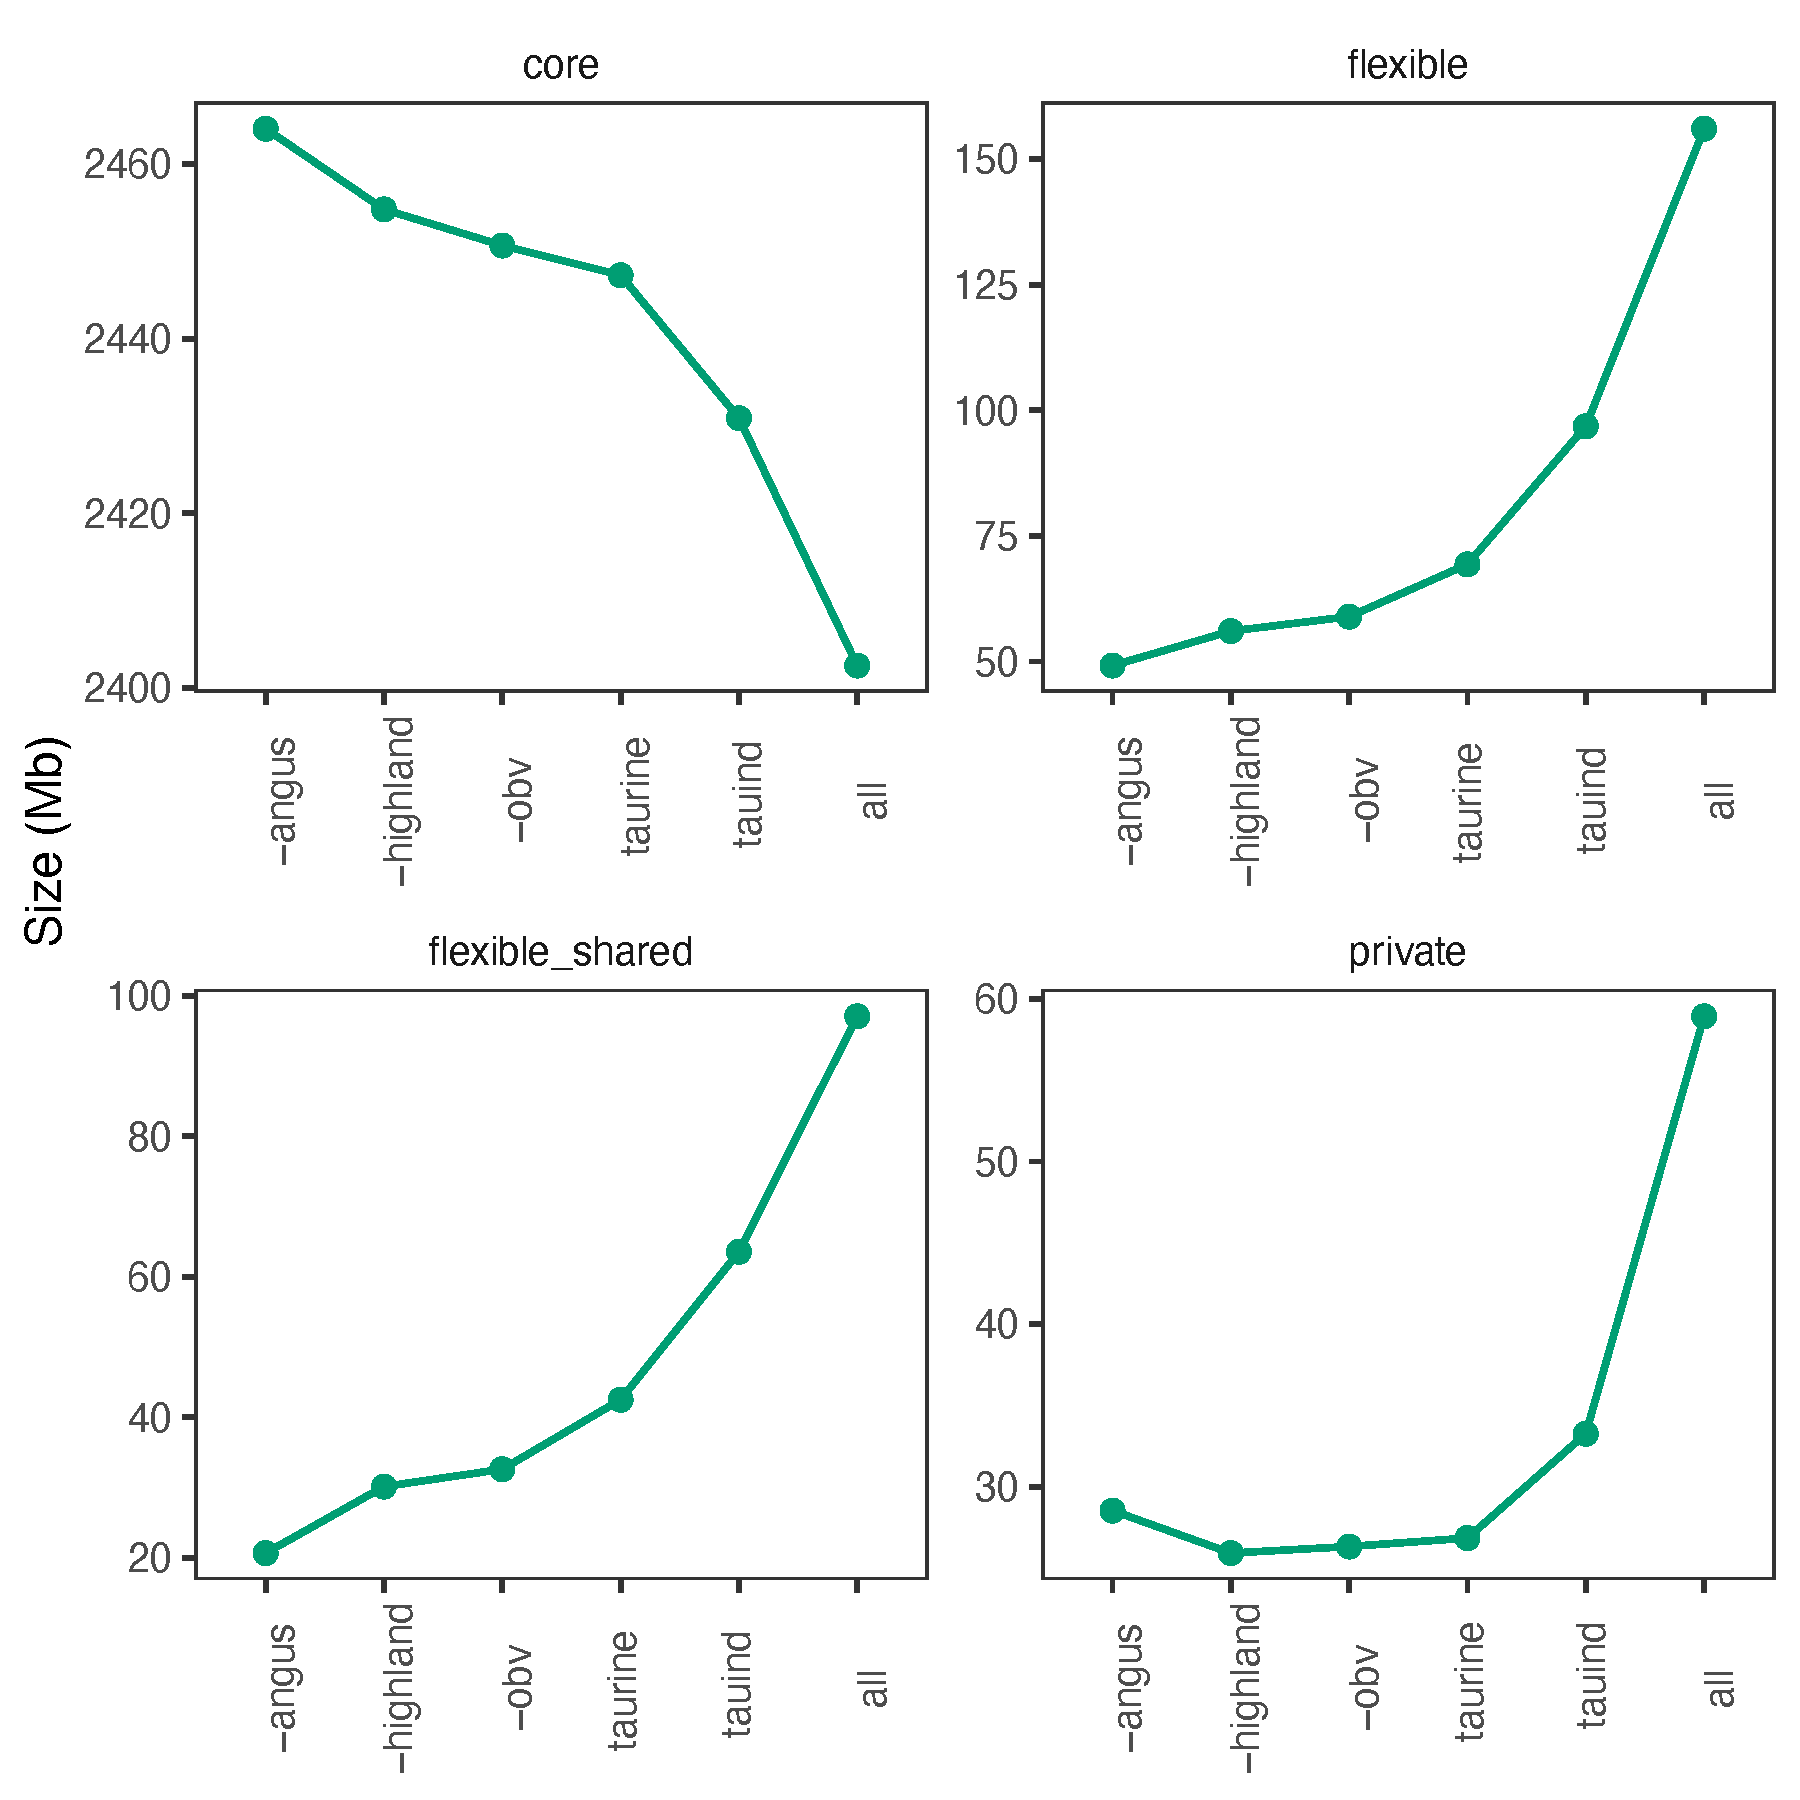
\includegraphics[width=0.8\textwidth]{paper3/supplement/sp416.pdf}
    \caption*{\textbf{\hypertarget{Figure SN42}{Figure SN42}: Pangenome profile as more distant assemblies are added to the graph.} \\
    \footnotesize{The X-axis indicates the constructed graphs (- denotes the taurine assembly that was removed from the taurine-only graph, taurine denotes a graph with four taurine assemblies, the indicine graph contains all taurine assemblies and the assembly of Brahman, and all reflects a multi-assembly graph that contains all six assemblies (taurine, indicine, and yak). The core part is the size of the segments that are common to all assemblies, flexible\_shared indicates the size of segments shared by at least two but not all assemblies, and private denotes the size of segments found only in a single assembly, thus flexible genome is composed of flexible\_shared + private segment.}}
\end{figure}


\subsection{}
\label{sup_not:s43}
\textbf{Construction of bovine multi-assembly graphs with different backbones}
\bigskip

To investigate if the choice of the backbone assembly influences the properties of the bovine multi-assembly graph, we constructed six graphs, one for each possible assembly backbone. The remaining five assemblies were added according to their Mash-distance to the chosen backbone. Larger assembly backbones tended to result in larger multi-assembly graphs (see Table 4.1 in the main paper, \hyperlink{Table SN4}{Table SN4}). The total number of non-reference bases detected varied between 63,745,420 bp and 72,349,303 bp for the OBV and Brahman backbone, with a mean value of 68.72 Mb and a standard deviation of 3.17 Mb. Fewer non-reference bases were detected when the OBV and Highland assemblies were used as backbones.
\bigskip

\textbf{\hypertarget{Table SN44}{Table SN44}: Properties of bovine multi-assembly graphs with different backbones}
\begin{center}
    \scriptsize
    \begin{tabular}{|c|c|c|c|c|c|c|c|}
    \hline
    \multirow{2}{*}{Parameter~} & \multirow{2}{*}{Unit} & \multicolumn{6}{c|}{Backbone Assembly}                                                         \\
    \cline{3-8}
                                &                       & Hereford      & Angus         & Highland      & OBV           & Brahman       & Yak            \\
    \hline
    Nodes                       & n                     & 182,940       & 182,332       & 183,118       & 184,098       & 184,301       & 188,975        \\
    \hline
    Size~                       & bp                    & 2,558,596,439 & 2,540,507,180 & 2,550,176,720 & 2,671,491,862 & 2,549,613,449 & 2,547,048,782  \\
    \hline
    Ref nodes~                  & n                     & 123,483       & 123,116       & 124,220       & 125,088       & 124,410       & 126,883        \\
    \hline
    Ref length~                 & bp                    & 2,489,385,779 & 2,468,157,877 & 2,483,452,092 & 2,607,746,442 & 2,478,073,158 & 2,478,308,164  \\
    \hline
    Nonref~nodes~               & n                     & 59,457        & 59,216        & 58,898        & 59,010        & 59,891        & 62,092         \\
    \hline
    Non-ref length~             & bp                    & 69,210,660    & 72,349,303    & 66,724,628    & 63,745,420    & 71,540,291    & 68,740,618     \\
    \hline
    Edges~                      & n                     & 258396        & 257531        & 258608        & 260044        & 260209        & 266139         \\
    \hline
    Edges/nodes~                & ratio                 & 1.4125        & 1.4124        & 1.4122        & 1.4125        & 1.4119        & 1.4083         \\
    \hline
    R-R~edges                   & n                     & 141,086       & 140,742       & 142,133       & 143,133       & 141,978       & 144,442        \\
    \hline
    R-NR~edges                  & n                     & 113,332       & 112,669       & 113,116       & 114,058       & 114,064       & 114,837        \\
    \hline
    NR-NR~edges                 & n                     & 3,978         & 4,120         & 3,359         & 2,853         & 4,167         & 6,860          \\
    \hline
    core count~                 & n                     & 67,482        & 67,499        & 67,616        & 67,619        & 67,763        & 68,614         \\
    \hline
    core length~                & bp                    & 2,402,561,410 & 2,394,756,562 & 2,402,656,874 & 2,414,762,810 & 2,398,150,572 & 2,397,494,177  \\
    \hline
    core prop~                  & \%                    & 93.9          & 94.26         & 94.22         & 90.39         & 94.06         & 94.13          \\
    \hline
    flexible count~             & n                     & 115,458       & 114,833       & 115,502       & 116,479       & 116,538       & 120,361        \\
    \hline
    flexible length~            & bp                    & 156,035,029   & 145,750,618   & 147,519,846   & 256,729,052   & 151,462,877   & 149,554,605    \\
    \hline
    flexible prop~              & \%                    & 6.10          & 5.74          & 5.78          & 9.61          & 5.94          & 5.87           \\
    \hline
    CPU time~                   & min                   & 290.43        & 276.33        & 274.52        & 210.46        & 282.59        & 299.01         \\
    \hline
    Max mem~                    & Gb                    & 55.03         & 58.88         & 55.6          & 58.31         & 56.67         & 56.96          \\
    \hline
    Average mem~                & Gb                    & 36.34         & 37.08         & 34.43         & 34.38         & 36.08         & 34.64          \\
    \hline
    Run Time~                   & min                   & 41.78         & 39.4          & 41.23         & 30.6          & 39.35         & 42.7           \\
    \hline
    \end{tabular}
\end{center}

\bigskip
\normalsize

The choice of the backbone had, as expected, a major impact on the amount of non-reference bases detected from each of the remaining assemblies (\hyperlink{Table SN45}{Table SN45}). A multi-assembly graph with a Bos taurus taurus backbone contains between 10.14 and 19.48 million non-reference bases from the remaining three taurine assemblies. Using the Hereford or Angus assemblies as the backbone resulted in more total non-reference sequences than using the OBV or Highland assemblies. Regardless of backbone choice, the OBV and Highland assemblies also contribute more non-reference sequences to the multi-assembly graph than the Hereford and Angus assembly. These two observations suggest that the OBV and Highland assemblies represent a more comprehensive \emph{Bos taurus taurus} genome, agreeing well with their high completeness, continuity, and correctness (see \ref{sup_not:s41} and \citep{rice2020continuous}). Thus, there is a tendency to detect fewer non-reference sequences with a more complete and contiguous backbone. Although selecting a more distant assembly as the backbone identifies more non-reference sequences from each remaining assembly on average (~40 Mb with Yak compared to ~20 Mb for taurine), this appeared to be a smaller effect compared to the backbone completeness.

\bigskip

\textbf{\hypertarget{Table SN45}{Table SN45}: : Non-reference bases detected (Mb)}
\begin{center}
    \begin{tabular}{|c|c|c|c|c|c|c|c|}
    \hline
    \multirow{2}{*}{Backbone~} & \multicolumn{7}{c|}{Assembly}                                       \\
    \cline{2-8}
                               & Hereford~ & Yak~  & Brahman~ & OBV~  & Angus~ & Highland~ & Total1  \\
    \hline
    Hereford~                  & -         & 43.34 & 23.64    & 18.2  & 14.45  & 15.54     & 69.21   \\
    \hline
    Yak~                       & 40.88     & -     & 40.12    & 44    & 38.94  & 39.48     & 68.74   \\
    \hline
    Brahman~                   & 23.09     & 42.11 & -        & 24.62 & 21.23  & 21.7      & 71.54   \\
    \hline
    OBV~                       & 11.91     & 39.64 & 17.69    & -     & 10.14  & 11.18     & 63.75   \\
    \hline
    Angus~                     & 17.99     & 44.02 & 23.40    & 19.48 & -      & 16.94     & 72.35   \\
    \hline
    Highland~                  & 13.03     & 40.09 & 20.27    & 14.21 & 11.64  & -         & 66.72   \\
    \hline
    \end{tabular}
\end{center}

\bigskip
\normalsize

Furthermore, the total length of each assembly’s private non-reference nodes, was barely affected by backbone choice. This suggests that our approach to building multi-assembly graphs with minigraph and labelling non-reference nodes work well regardless of choice of the initial backbone assembly (\hyperlink{Table SN46}{Table SN46}).

\bigskip

\textbf{\hypertarget{Table SN46}{Table SN46}: Total length in Mb of private non-reference nodes.}
\begin{center}
    \begin{tabular}{|c|c|c|c|c|c|c|}
    \hline
    \multirow{2}{*}{Backbone~} & \multicolumn{6}{c|}{Assembly}                             \\
    \cline{2-7}
                               & Hereford~ & Yak~  & Brahman~ & OBV~ & Angus~ & Highland~  \\
    \hline
    Hereford~                  & -         & 29.9  & 8.22     & 4.61 & 2.39   & 2.78       \\
    \hline
    Yak~                       & 4.36      & -     & 8.62     & 5.05 & 2.47   & 2.93       \\
    \hline
    Brahman~                   & 4.69      & 30.26 & -        & 4.85 & 2.69   & 3.19       \\
    \hline
    OBV~                       & 4.33      & 30.02 & 8.34     & -    & 2.67   & 3.02       \\
    \hline
    Angus~                     & 4.60      & 29.85 & 8.20     & 5.01 & -      & 2.76       \\
    \hline
    Highland~                  & 4.40      & 29.85 & 8.14     & 4.75 & 2.38   & -          \\
    \hline
    \end{tabular}
\end{center}
\newpage

\textbf{Assessment of the sequences not included in the graphs}

Minigraph might fail to align and include input sequences into the graph. We assessed bases not included in the graph by comparing the total realignment size of the assembly to the graphs with the total pangenome size. All bases in the backbone are included in the multi-assembly graph, but this is not the case for the additional assemblies which subsequently augment the graph (\hyperlink{Table SN47}{Table SN47}). We again found that the use of the Original Braunvieh backbone led to fewer non-reference bases not included in the graph from each remaining assembly.

\bigskip

\textbf{\hypertarget{Table SN47}{Table SN47}: Total assembly sequences (bp) not included in the graphs.}
\begin{center}
    \centering
    \footnotesize
    \begin{tabular}{|l|l|l|l|l|l|l|l|} 
    \hline
    \multicolumn{1}{|c|}{\multirow{2}{*}{Backbone~}} & \multicolumn{6}{c|}{Assembly}                                                & \multicolumn{1}{c|}{\multirow{2}{*}{Total}}  \\ 
    \cline{2-7}
    \multicolumn{1}{|c|}{}                            & Hereford~  & Yak        & Brahman ~  & OBV         & Angus      & Highland   & \multicolumn{1}{c|}{}                        \\ 
    \hline
    Hereford                                          & -          & 5,388,777  & 6,369,649  & 106,905,680 & 7,442,463  & 8,165,867  & 134,272,436~                                 \\ 
    \hline
    Yak                                               & 15,420,157 & -          & 9,466,221  & 116,311,772 & 8,286,464  & 10,732,937 & 160,217,551~                                 \\ 
    \hline
    Brahman~                                          & 17,427,243 & 9,103,978  & -          & 111,856,939 & 12,067,771 & 12,108,523 & 162,564,454~                                 \\ 
    \hline
    OBV                                               & 9,716,932  & 2,690,446  & 3,339,031  & -           & 882,571    & 4,659,329  & 21,288,309~                                  \\ 
    \hline
    Angus                                             & 26,973,081 & 18,470,665 & 20,032,971 & 115,587,224 & -          & 20,796,186 & 201,860,127~                                 \\ 
    \hline
    Highland                                          & 13,401,923 & 6,069,608  & 7,053,961  & 104,868,806 & 6,680,628  & -          & 138,074,926~                                 \\
    \hline
    \end{tabular}
\end{center}

\bigskip

The Original Braunvieh assembly has between 105 and 116 Mb of sequences which are not augmented into the different multi-assembly graphs. We investigated which parts of the OBV assembly were not included in the Hereford-backbone graph using the reverse mapping approach enumerated below:

\bigskip

\begin{enumerate}
    \item Extract nodes in the graph covered with OBV alignment
    \item Map the sequence in the node to the OBV assembly using minimap2
    \item Collect region longer than 10kb with no coverage from the alignment
    \item Visualize the region across OBV genome region
\end{enumerate}

\bigskip

As shown in \hyperlink{Figure SN43}{Figure SN43}, many sequences not included in the graph are located at the start or end of chromosomes, which might indicate that the HiFi reads enabled a better (more complete) assembly of telomeric or centromeric regions. This hypothesis is further supported by a repeatmasker analysis revealing that these regions contain many DNA satellite (21,139,818 bp) and retroelements (7,774,559 bp).

\bigskip
\begin{figure}[!htb]
    \centering
    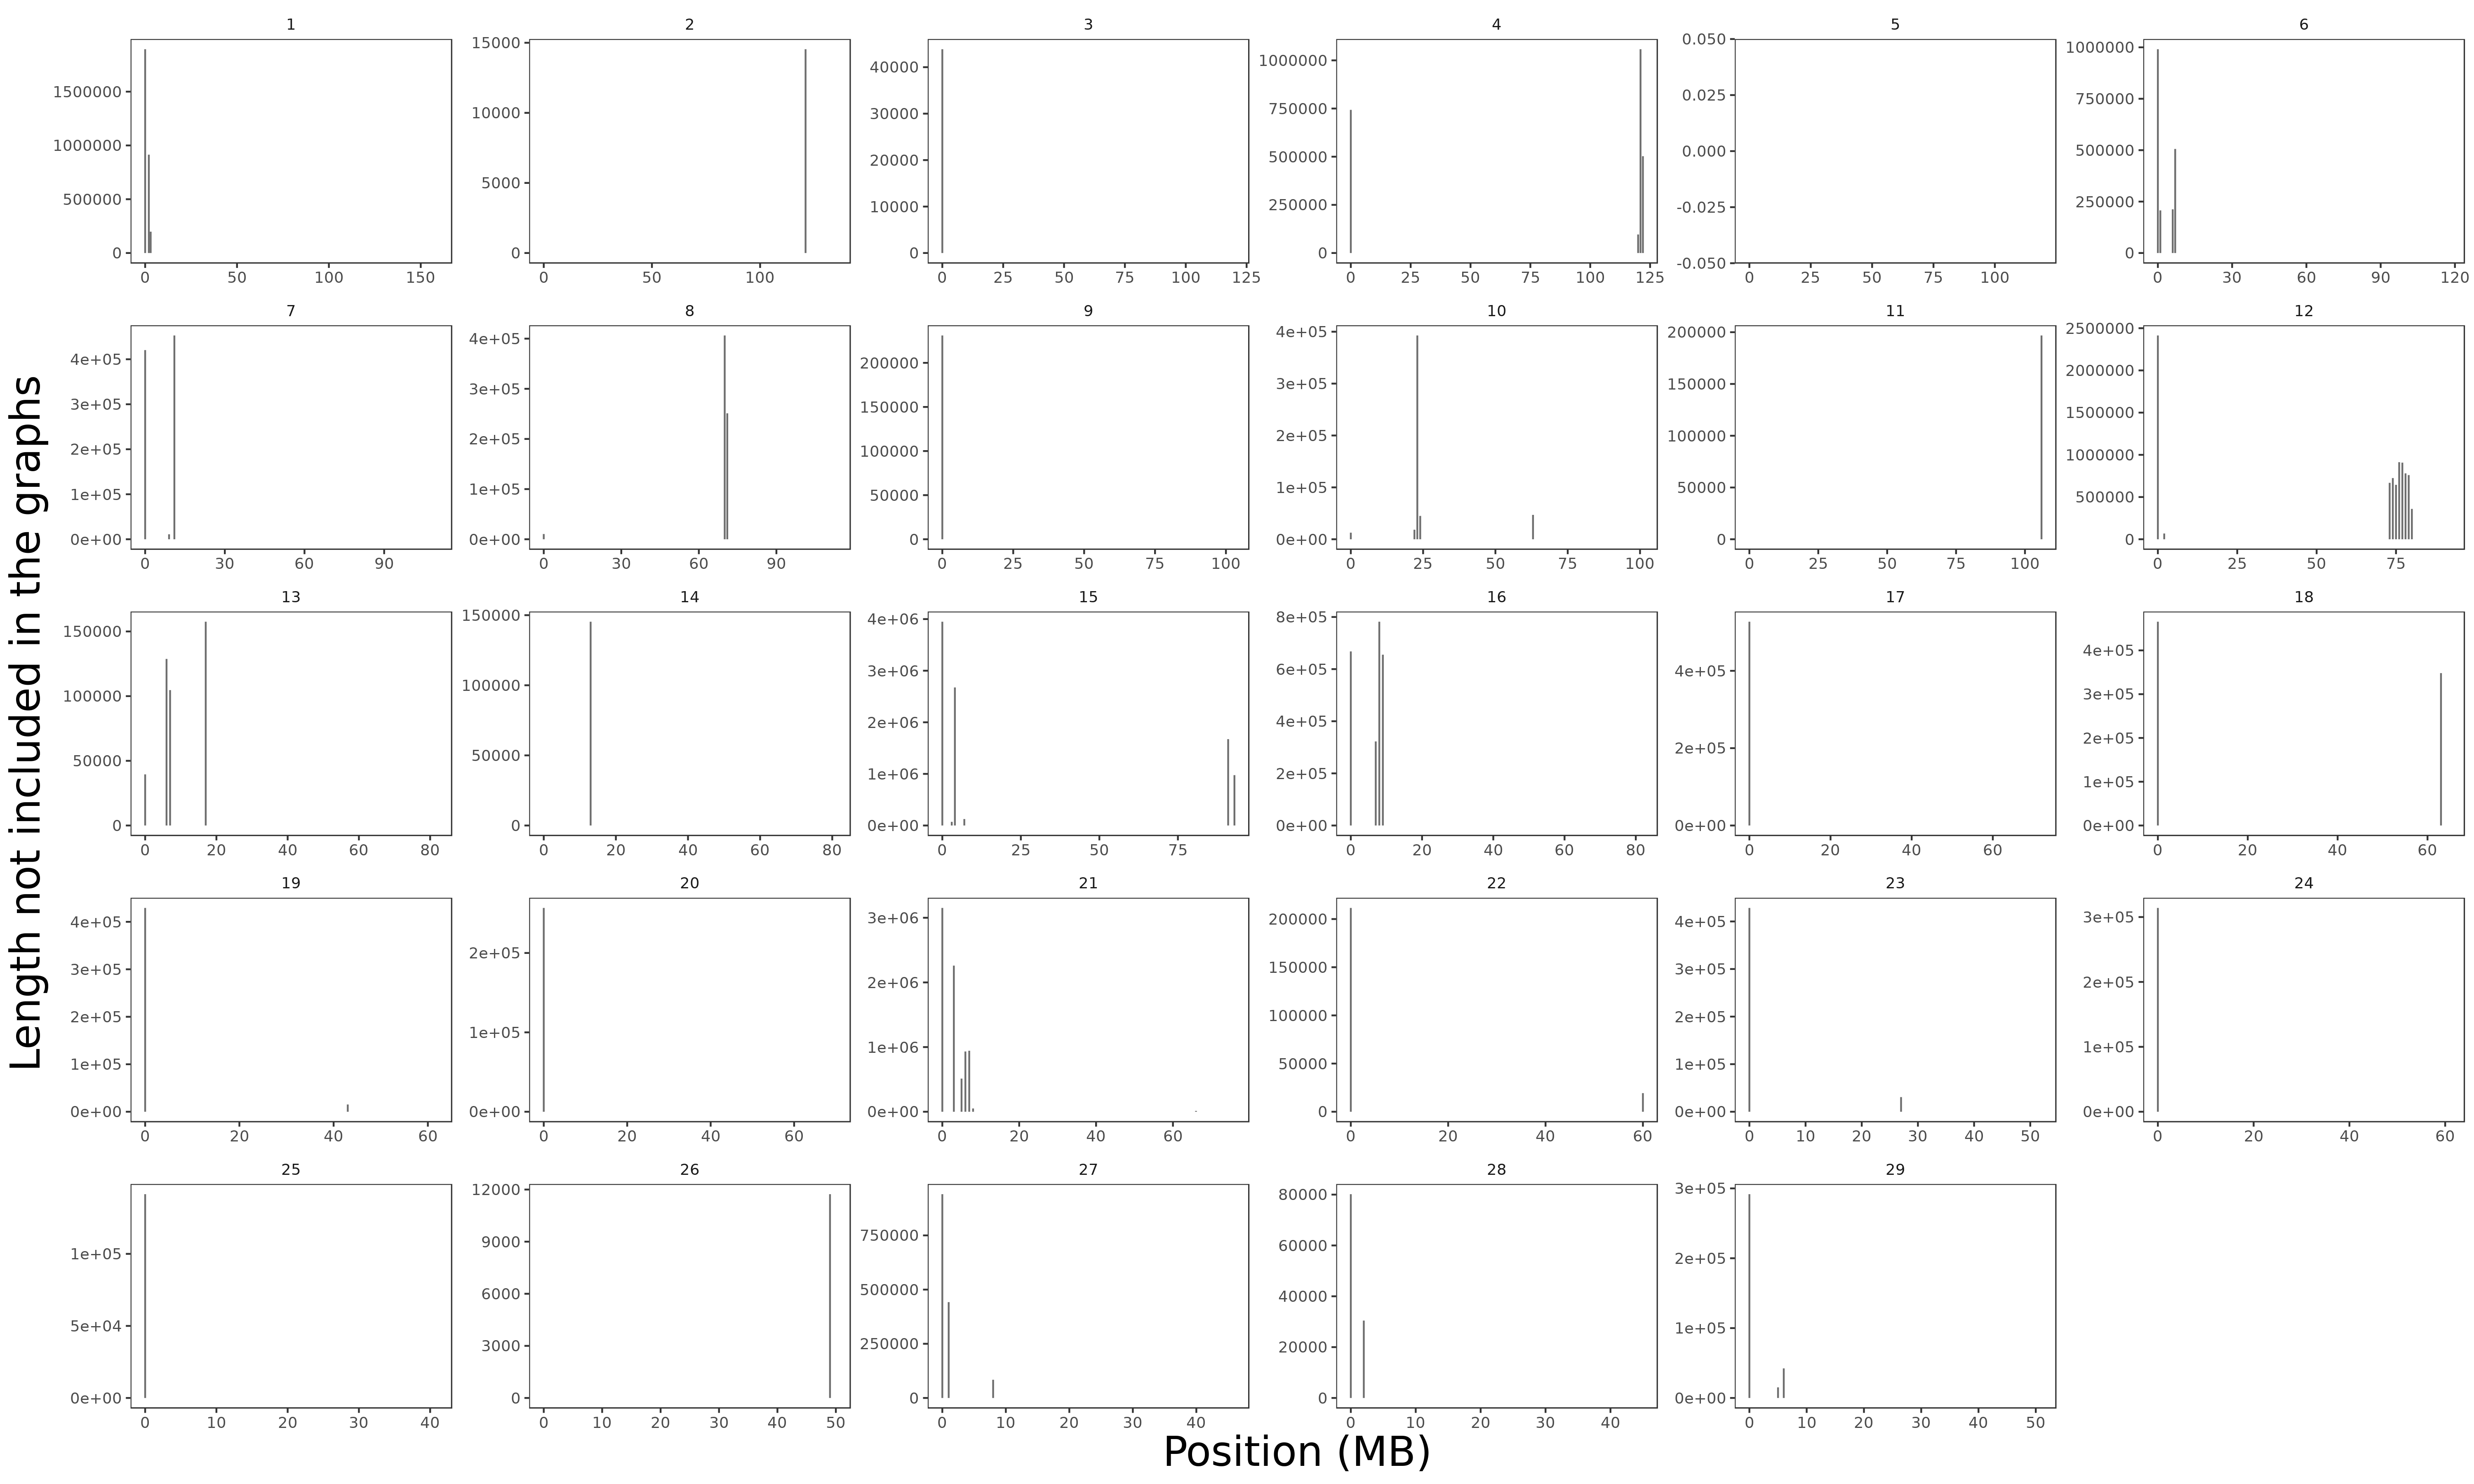
\includegraphics[width=\textwidth]{paper3/supplement/sp417.png}
    \caption*{\textbf{\hypertarget{Figure SN43}{Figure SN43}: The location of sequences from the Original Braunvieh assembly not included in the graph.} Numbers above the plot denote chromosomal identifiers.}
\end{figure}

\clearpage

\subsection{}
\label{sup_not:s44}
\textbf{Differential expression analysis}
\bigskip

We tested 13,085 genes that were expressed $>=$ 1 CPM in at least eight samples (sample size from each group) for differential expression between \emph{Mycobacterium bovis}-infected and non-infected control animals. We detected (adjusted FDR $≤$ 0.05) 1,769 and 1,877 genes that were up-and down-regulated respectively in peripheral blood leukocytes of \emph{Mycobacterium bovis}-infected cattle (\hyperlink{Figure SN44}{Figure SN44}). Of 12,813 genes of the Ensembl ARS-UCD1.2 genome annotation that were expressed at $>=$1 CPM in at least eight samples, 3610 (28.17\%) were differentially expressed. Of 272 putatively novel genes that were expressed $>=$1 CPM in at least 8 samples, 36 (13.23\%) were differentially expressed.

\bigskip


We found that genes relevant for the immune response were among the top differentially expressed genes with the greatest mean log-fold change (e.g., DEFB10 -8.24-fold, CXCL10 -3.30-fold, IL12B -3.11-fold, CXCL5 7.11-fold, CTLA4 4.25-fold, and CXCL8 5.70-fold), matching observations on an older reference genome annotation by McLoughlin \emph{et al.} \hyperlink{Table SN8}{Table SN8}. Multidimensional scaling (MDS) representations of transcript abundance estimates from either all 13,085 genes (\hyperlink{Figure SN45}{Figure SN45}b) or 3646 differentially expressed genes (\hyperlink{Figure SN45}{Figure SN45}a) separated Mycobacterium bovis-infected from healthy cattle. We discovered more differentially expressed genes of the Ensembl ARS-UCD1.2 genome annotation than McLoughlin \emph{et al.} (3610 vs. 3250), likely due to a vastly improved genome assembly (27,115 vs. 24,616 genes are included in build 101 (ARS-UCD1.2) and build 73 (UMD3.1), respectively). Using data from the supplement provided by McLoughlin \emph{et. al}, we were able to compare the expression levels of 2678 (out of 3250) differentially expressed genes between different genome builds (UMD31, standard and extended ARS-UCD1.2) and annotations (\hyperlink{Figure SN46}{Figure SN46}). Six genes with the greatest fold-change increase in expression reported by McLoughlin \emph{et al.} had a very similar expression pattern from all assemblies considered.


\bigskip 

\textbf{\hypertarget{Table SN48}{Table SN48}: The expression of 6 immune genes reported by McLoughlin \emph{et al.} across different assemblies.}
\begin{center}
        \footnotesize
            \begin{tabular}{|l|l|l|l|l|} 
            \hline
            \multicolumn{1}{|c|}{\textbf{Ensembl gene ID}} & \multicolumn{1}{c|}{\textbf{Gene symbol}} & \multicolumn{1}{c|}{\begin{tabular}[c]{@{}c@{}}\textbf{Log2FC UMD3.1~}\\\textbf{(McLoughlin~\textit{et. al})}\end{tabular}} & \multicolumn{1}{c|}{\begin{tabular}[c]{@{}c@{}}\textbf{Log2FC~}\\\textbf{Standard}\\\textbf{ARS-UCD1.2}\end{tabular}} & \multicolumn{1}{c|}{\begin{tabular}[c]{@{}c@{}}\textbf{Log2FC~}\\\textbf{Extended}\\\textbf{ARS-UCD1.2}\end{tabular}}  \\ 
            \hline
            ENSBTAG00000019716                             & CXCL8                                     & 2.435                                                                                                                       & 2.512                                                                                                                 & 2.512                                                                                                                  \\ 
            \hline
            ENSBTAG00000009812                             & CXCL5                                     & 2.763                                                                                                                       & 2.831                                                                                                                 & 2.831                                                                                                                  \\ 
            \hline
            ENSBTAG00000013170                             & CTLA4                                     & 1.849                                                                                                                       & 2.088                                                                                                                 & 2.088                                                                                                                  \\ 
            \hline
            ENSBTAG00000004741                             & IL12B                                     & -2.129                                                                                                                      & -1.841                                                                                                                & -1.841                                                                                                                 \\ 
            \hline
            ENSBTAG00000048737                             & DEFB10                                    & -2.850                                                                                                                      & -3.042                                                                                                                & -3.042                                                                                                                 \\ 
            \hline
            ENSBTAG00000001725                             & CXCL10                                    & -1.712                                                                                                                      & -1.722                                                                                                                & -1.722                                                                                                                 \\
            \hline
        \end{tabular}
\end{center}

\bigskip
\begin{figure}[!htb]
    \centering
    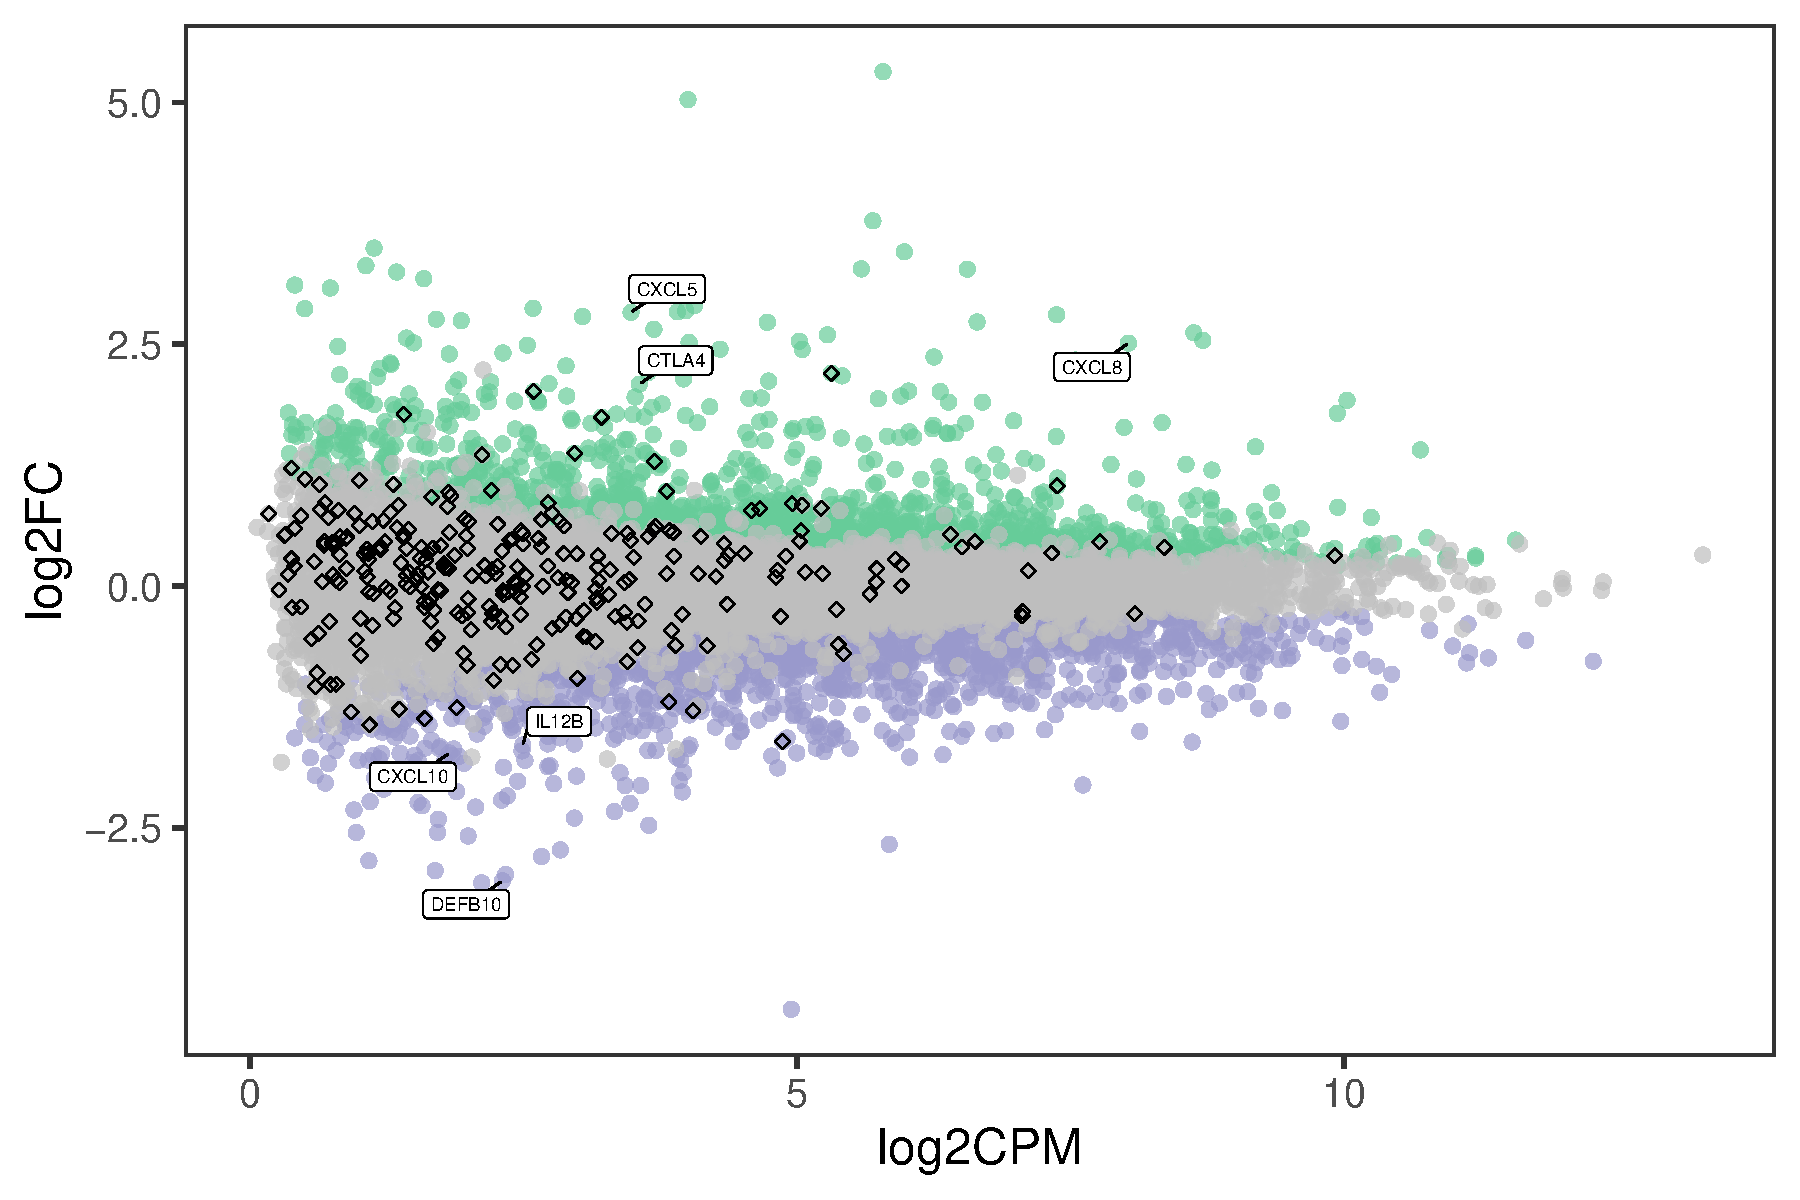
\includegraphics[width=\textwidth]{paper3/supplement/sp418.pdf}
    \caption*{\textbf{\hypertarget{Figure SN44}{Figure SN44}: Smear plot from the differential expression analysis.} Grey, green, and purple color indicates genes with no expression difference, significant up-regulation, and down-regulation in peripheral blood leukocytes of \emph{ Mycobacterium bovis}-infected cattle. Diamonds indicate 272 putatively novel genes assembled from RNA sequencing reads mapping to non-reference sequences. Six genes reported by (McLoughlin \emph{ et al.} 2014) are indicated with the text labels.}
\end{figure}

\bigskip
\begin{figure}[!htb]
    \centering
    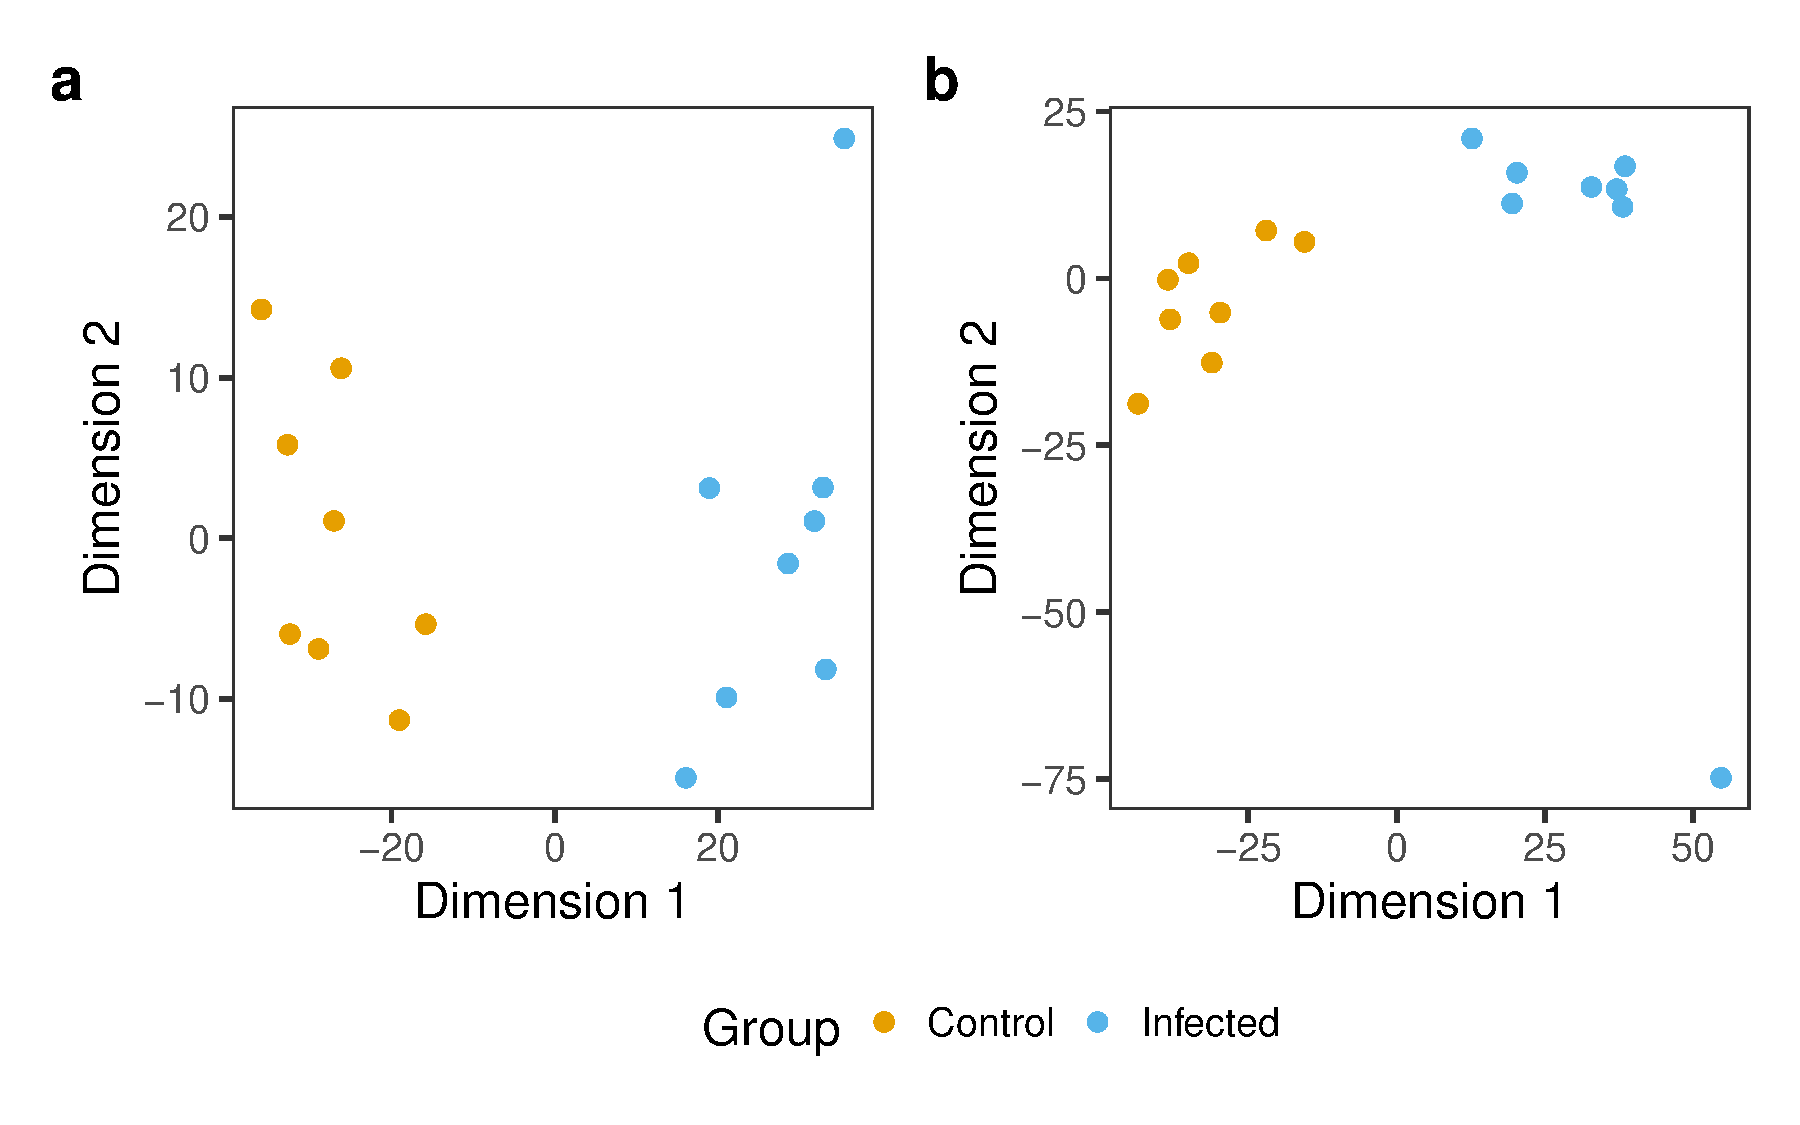
\includegraphics[width=\textwidth]{paper3/supplement/sp419.pdf}
    \caption*{\textbf{\hypertarget{Figure SN45}{Figure SN45}: Multidimensional scaling analysis (MDS) based on transcript abundance estimates of (a) 3646 differentially expressed, and (b) 13,085 genes with CPM$>=$1 in eight samples.} Each point represents an individual \emph{Mycobacterium bovis}-infected (blue) or control (orange) sample.}
\end{figure}

\bigskip
\begin{figure}[!htb]
    \centering
    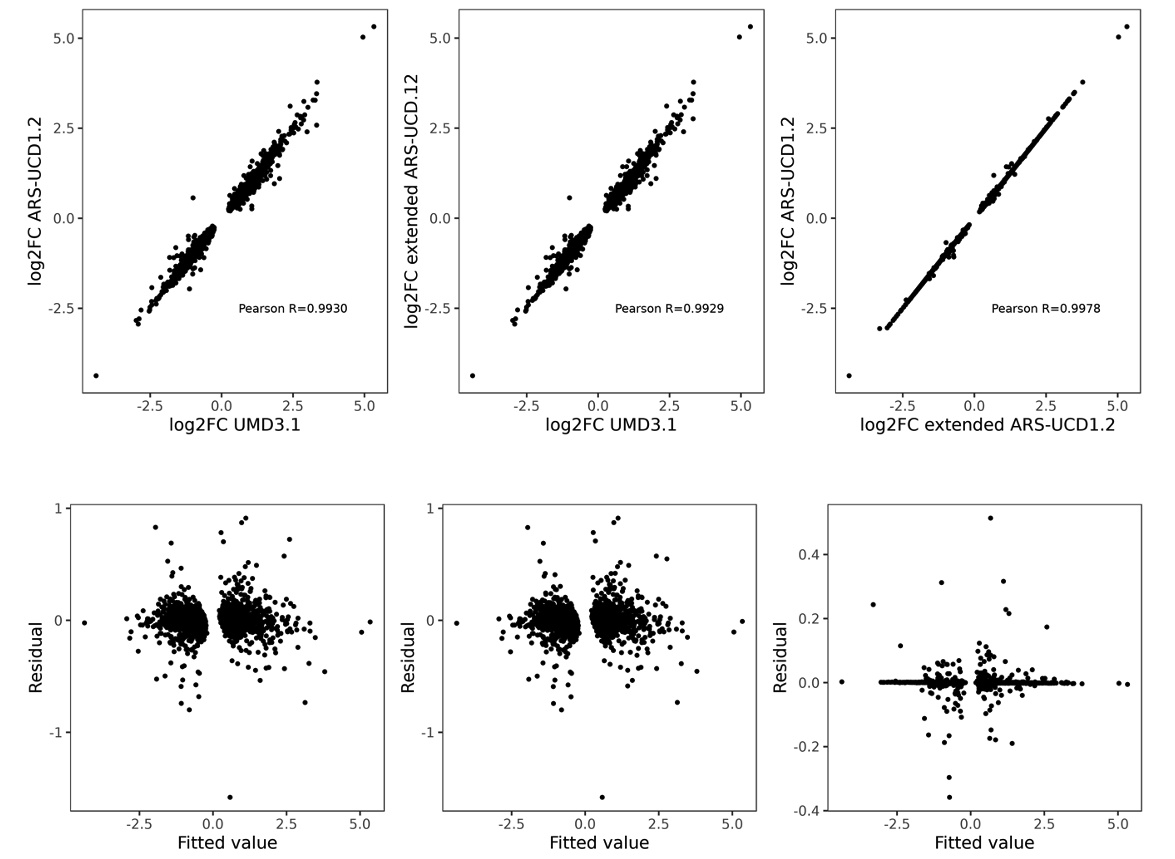
\includegraphics[width=\textwidth]{paper3/supplement/sp420.png}
    \caption*{\textbf{\hypertarget{Figure SN46}{Figure SN46}: Log2FC expression of 2678 genes between UMD3.1 (as reported in McLoughlin \emph{et. al}), the standard ARS-UCD1.2, and extended ARS-UCD1.2 reference.} Each point indicates the expression of a gene.}
\end{figure}

\clearpage

\subsection{}
\label{sup_not:s45}
\textbf{Detailed description of the analysis workflow presented in the main paper}
\bigskip

Step by step (manual) instruction to construct a multi-assembly graph from a collection of genome assemblies and characterize its structural variations. All steps can be automatically invoked with a workflow from a Github repository (\url{https://github.com/AnimalGenomicsETH/bovine-graphs}). \\ 
\bigskip 
\emph{Pangenome graph construction}

\bigskip 

1. Estimate pairwise genetic distance between the assemblies. \\
    \begin{figure}[!htb]
        \centering
        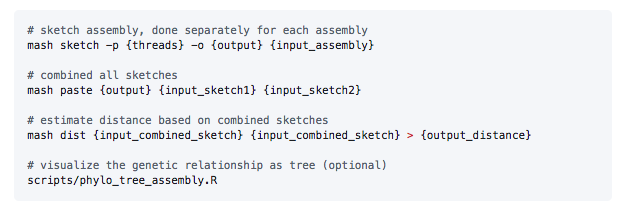
\includegraphics[width=\textwidth]{paper3/supplement/sp421.png}
    \end{figure}
2. Graph construction \\ Assemblies are added to the graph based on their genetic distance to the backbone assembly. Less distant assemblies are added before the more distant ones. \\
    \begin{figure}[!htb]
        \centering
        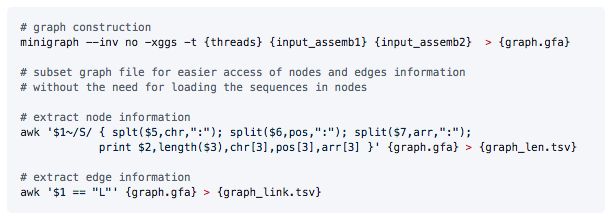
\includegraphics[width=\textwidth]{paper3/supplement/sp422.png}
    \end{figure}
3. Re-align each assembly to the multi-assembly graph \\ Separately realign each assembly to the multi-assembly graph to record the coverage for all nodes and edges in the graph. \\
    \begin{figure}[!htb]
        \centering
        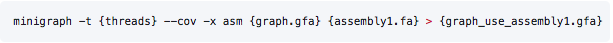
\includegraphics[width=\textwidth]{paper3/supplement/sp423.png}
    \end{figure}
    \newpage
4. Combine node and edge coverage across assemblies. \\
    \begin{figure}[!htb]
        \centering
        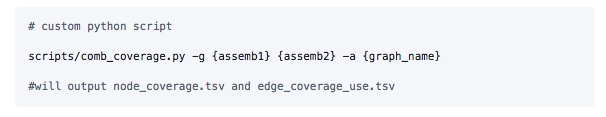
\includegraphics[width=\textwidth]{paper3/supplement/sp424.png}
    \end{figure}
5. Use coverage data to label the nodes in the graph. \\
    \begin{figure}[!htb]
        \centering
        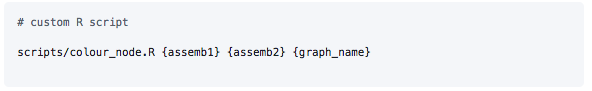
\includegraphics[width=\textwidth]{paper3/supplement/sp425.png}
    \end{figure}

6. Analyze the properties of the multi-assembly graph based on the node and edge labels. \\
    \begin{figure}[!htb]
        \centering
        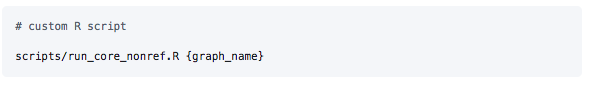
\includegraphics[width=\textwidth]{paper3/supplement/sp426.png}
    \end{figure}

\bigskip

\emph{Structural variations analysis}

\bigskip
1. Identify bubbles in the graph \\ Bubbles are regions that diverged between assemblies which have a common start and stop node derived from reference sequences. \\
\begin{figure}[!htb]
    \centering
    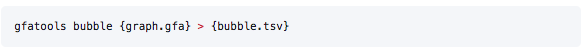
\includegraphics[width=\textwidth]{paper3/supplement/sp429.png}
\end{figure}

2. Identify the precise location of the structural variations from the multi-assembly graph \\ Paths in the bubble represent alleles of the structural variations. This step will enumerate all possible paths based on the start and stop node of the bubbles, done separately for biallelic (2 paths/alleles) and multi-allelic ($>=$3 alleles) bubbles. Finally, it labels structural variations according to the origin of the assemblies. \\
\begin{figure}[!htb]
    \centering
    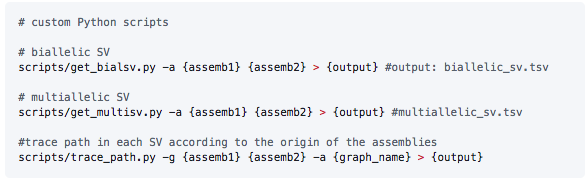
\includegraphics[width=\textwidth]{paper3/supplement/sp430.png}
\end{figure}

\newpage

3. Annotate the breakpoints detected in from the multi-assembly graph \\ Annotate the breakpoint of the structural variations using start and stop node coordinate for left and right breakpoints, respectively on the reference backbone coordinate. This step requires an annotation file from the backbone assembly. \\
\begin{figure}[!htb]
    \centering
    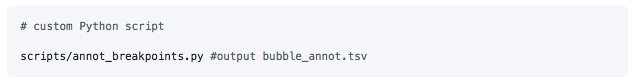
\includegraphics[width=\textwidth]{paper3/supplement/sp431.png}
\end{figure}

4. Extract structural variation alleles in the bubbles \\ Extract non-ref alleles (excluding paths less than 100 bp, complete deletions, or paths without non-ref sequences) as a representative non-reference sequences of the pangenome. Sequences in nodes are not used directly, because multiple consecutive nodes might be part of the same allele, and they are representing a continuous sequences. \\
\begin{figure}[!htb]
    \centering
    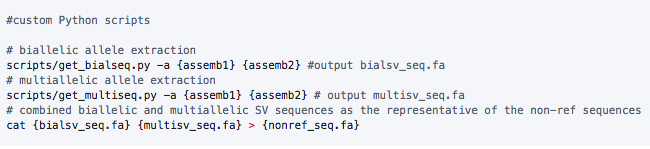
\includegraphics[width=\textwidth]{paper3/supplement/sp432.png}
\end{figure}


\renewcommand{\bibname}{Supplementary References}
\bibliographystyle{abbrvnat}
\bibliography{references/chapter4_ref}




\end{flushleft}

\ifdefined\BuildingFromMainFile
\else
   \end{document}
\fi
